%%=============================================================================
%% Resultaten
%%=============================================================================

\chapter{Resultaten}
\label{ch:resultaten}

\section{Analyse van de Trainingsfase}
\label{sec:train_analysis}

De trainingsopzet en trainingsloop (zie code) leiden tot de onderstaande trainingscurves voor elk model. Deze curves tonen het leer- en validatiegedrag tijdens training en worden gebruikt om vroege convergentie en mogelijke overfitting te identificeren.

\begin{listing}[H]
    \inputminted[fontsize=\footnotesize, linenos, frame=lines]{python}{code/training_loop.py}
    \caption{Python script voor de trainingsloop en evaluatiestructuur.}
    \label{lst:results_training_loop}
\end{listing}

Figuur \ref{fig:training_curves} toont de trainingscurves voor alle drie modellen op de DeepDetect-2025 dataset. Deze figuren illustreren de train- en validatieloss en de bijbehorende performance-metrieken per epoch.

\begin{figure}[H]
    \centering
    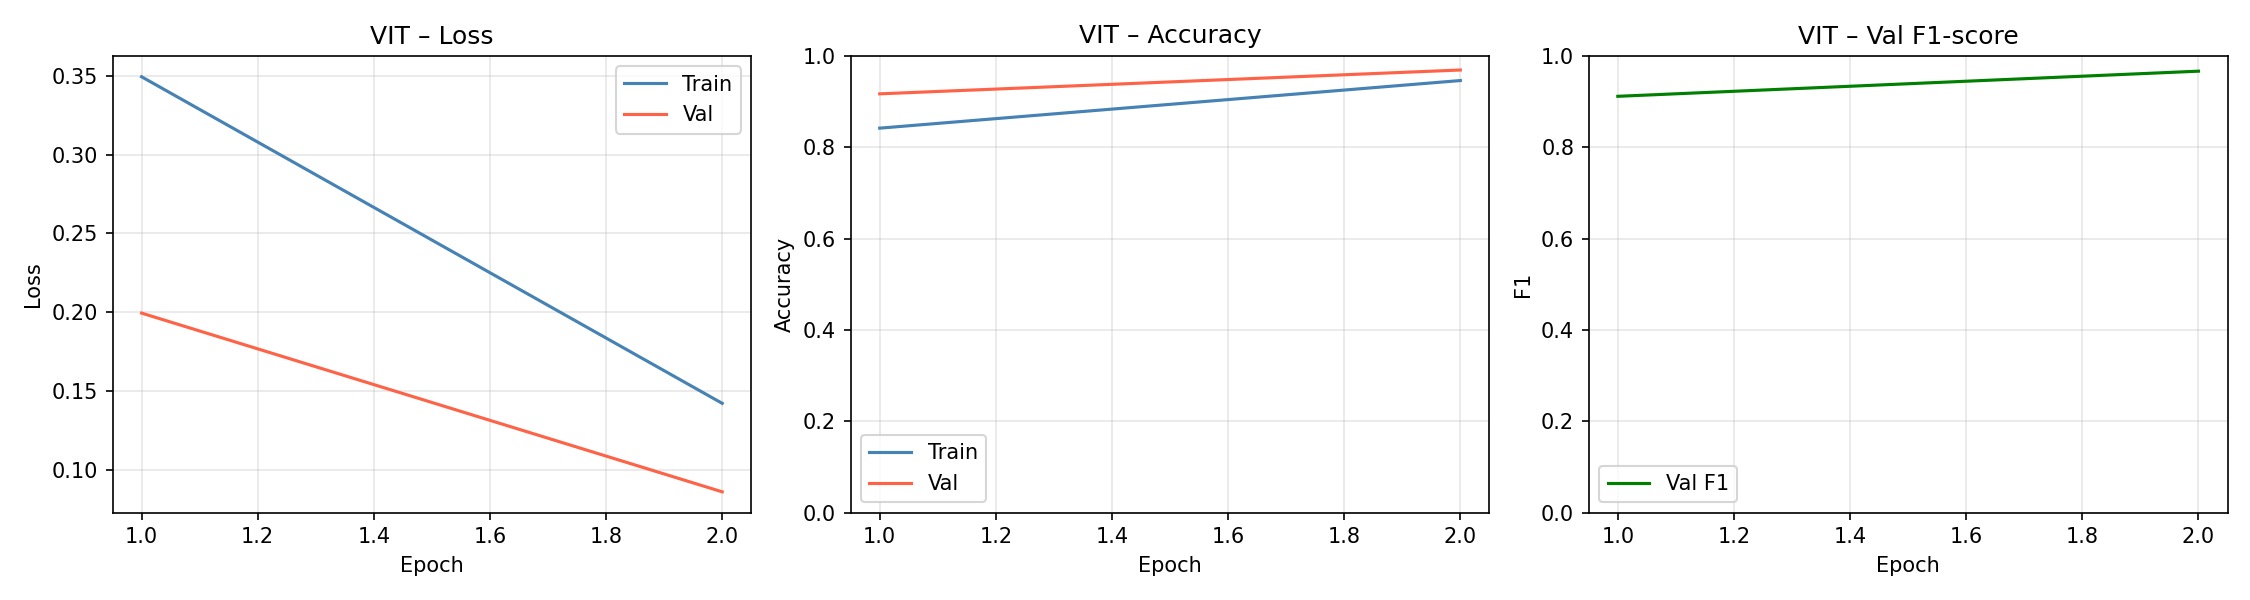
\includegraphics[width=0.9\textwidth]{../ipynb_output/ViT_results/training_curves.png}
    \centerline{\small (a) Training Curves voor ViT-Base/16 op DeepDetect-2025}
    
    \vspace{1cm}
    
    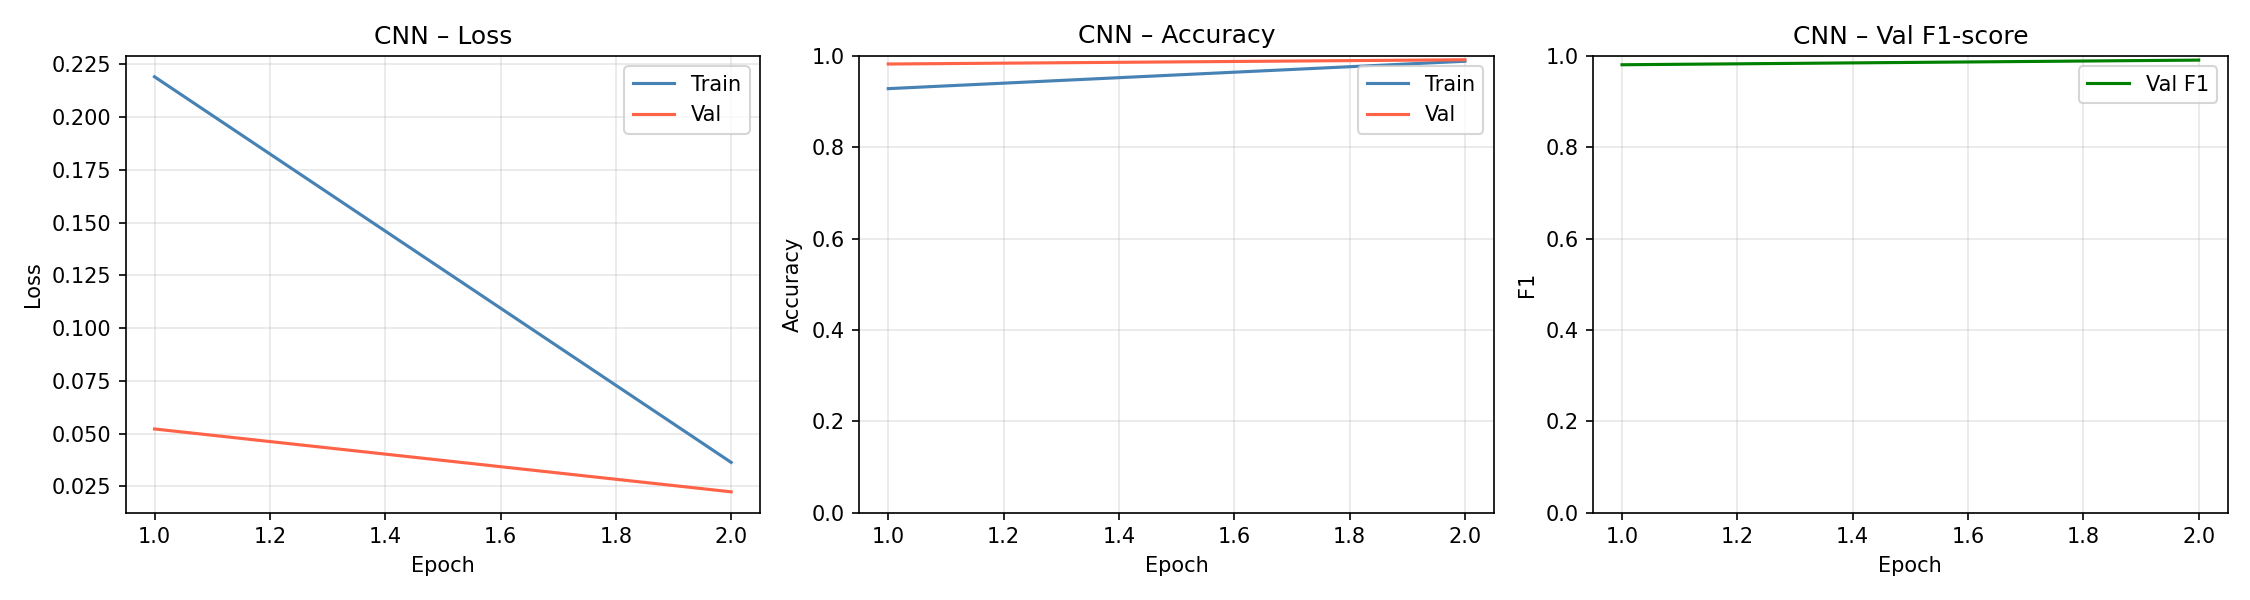
\includegraphics[width=0.9\textwidth]{../ipynb_output/CNN_results/training_curves.png}
    \centerline{\small (b) Training Curves voor CNN op DeepDetect-2025}

    \vspace{1cm}
    
    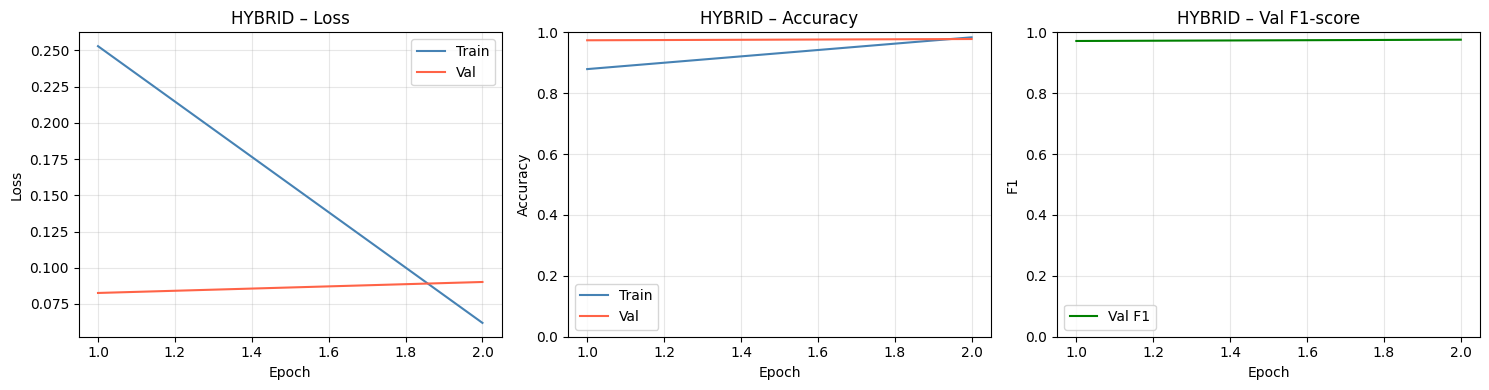
\includegraphics[width=0.9\textwidth]{../ipynb_output/Hybrid_results/training_curves.png}
    \centerline{\small (c) Training Curves voor Hybride model op DeepDetect-2025}
    
    \caption[Training Curves op DeepDetect-2025]{Training Curves voor de DeepDetect-2025 dataset.}
    \label{fig:training_curves}
\end{figure}

\section{Evaluatie en Cross-Dataset Generalisatie}
\label{sec:eval_generalisation}

Deze sectie bevat de kernresultaten: ROC- en PR-curves, confusion matrices, en vergelijkende metrics (accuracy en F1) tussen de interne testset (DeepDetect-2025) en de externe 140k Real and Fake Faces dataset.

\begin{figure}[H]
    \centering
    \begin{minipage}{0.48\textwidth}
        \centering
        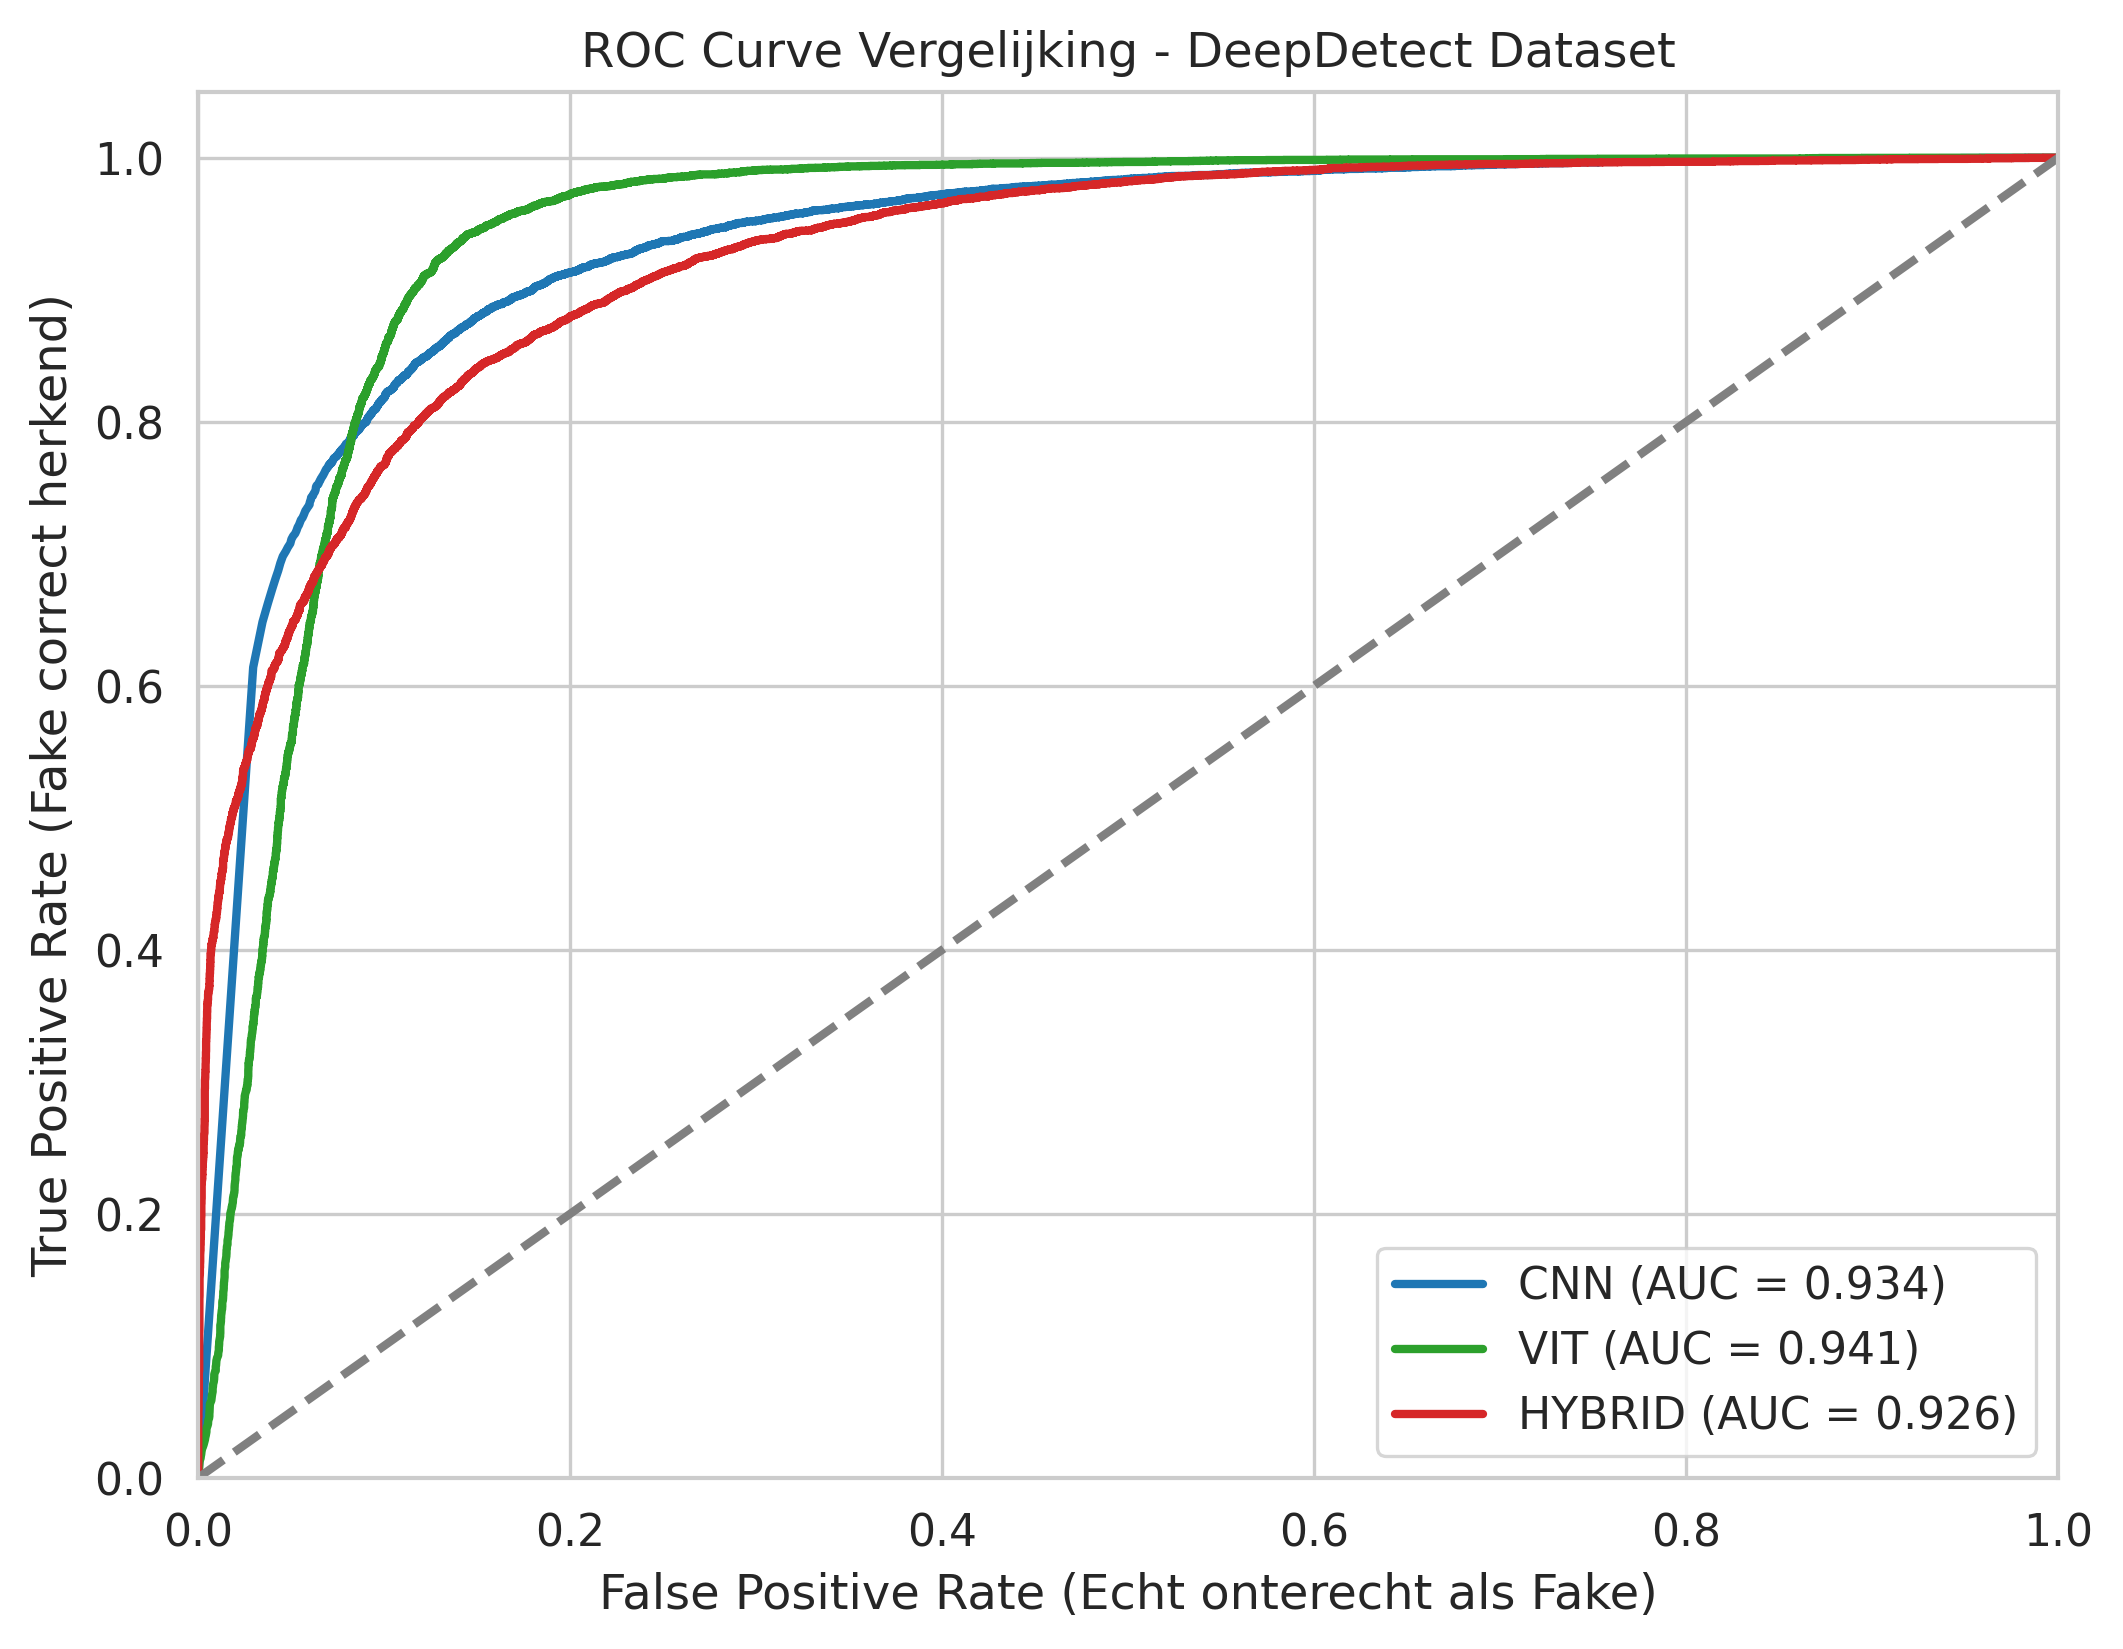
\includegraphics[width=\textwidth]{../ipynb_output/roc_pr/ROC_DeepDetect.png}
        \centerline{\scriptsize (a) ROC-curve op DeepDetect}
    \end{minipage}
    \hfill
    \begin{minipage}{0.48\textwidth}
        \centering
        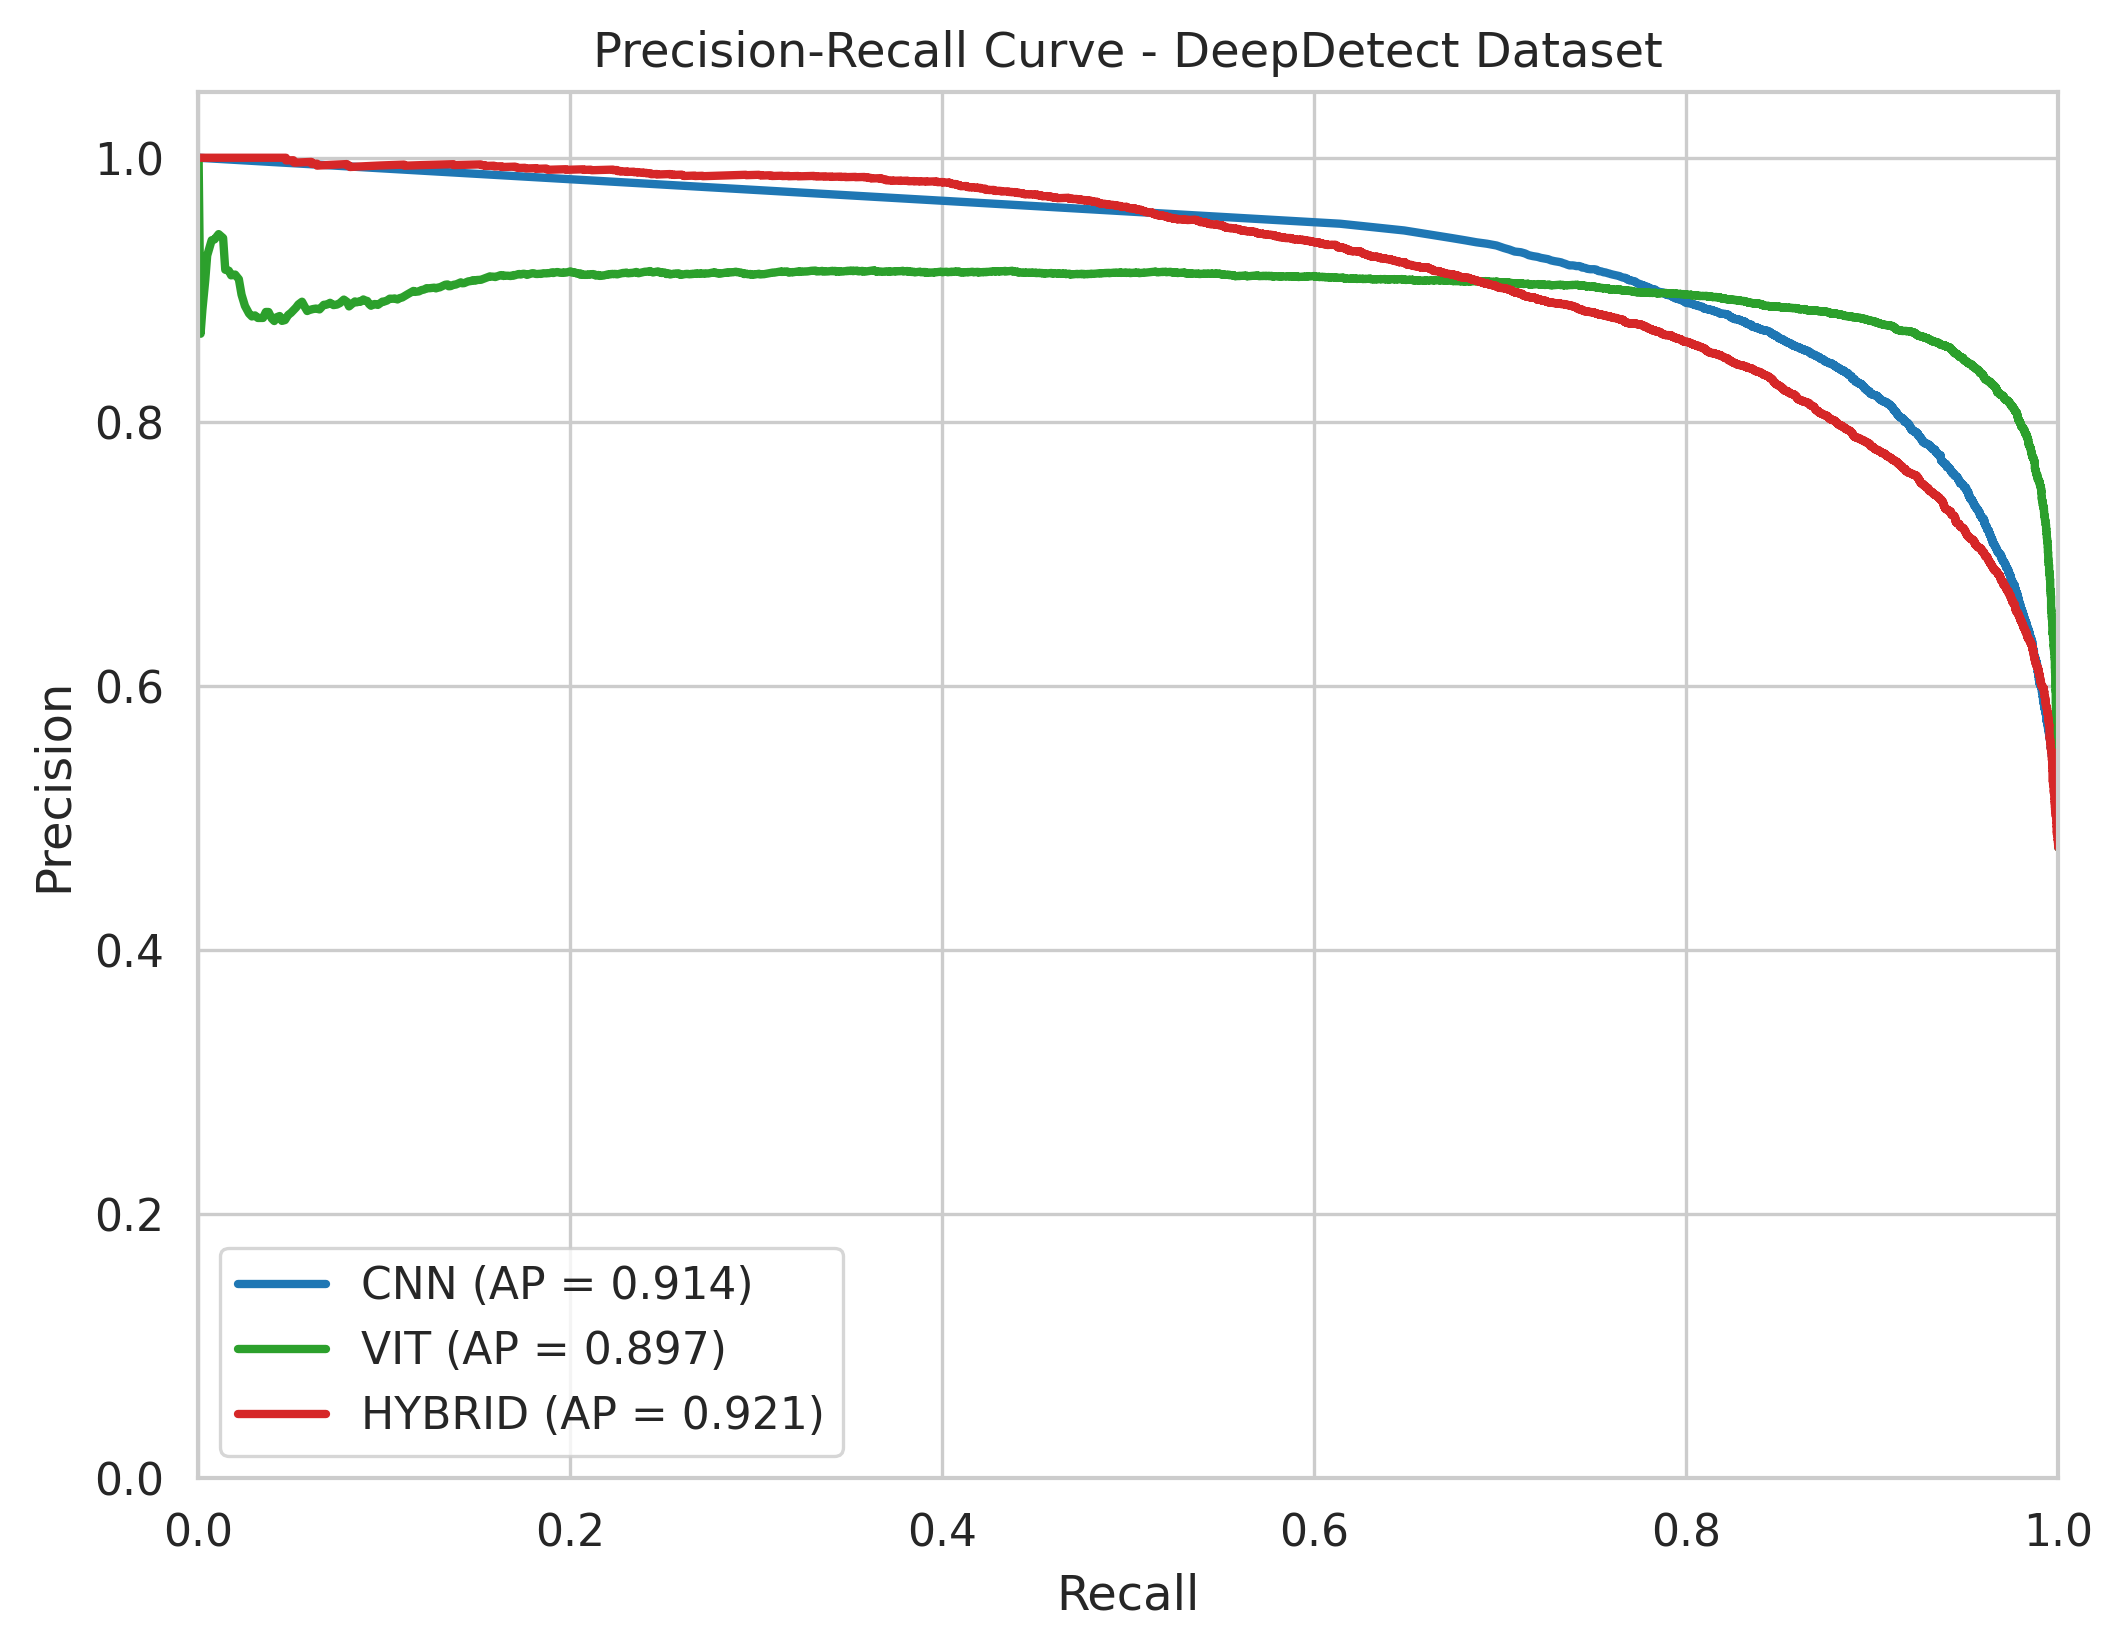
\includegraphics[width=\textwidth]{../ipynb_output/roc_pr/PR_DeepDetect.png}
        \centerline{\scriptsize (b) PR-curve op DeepDetect}
    \end{minipage}
    \caption[ROC- en PR-curves op DeepDetect]{ROC- en PR-curves voor de DeepDetect-2025 dataset.}
    \label{fig:roc_pr_deepdetect}
\end{figure}

\begin{figure}[H]
    \centering
    \begin{minipage}{0.48\textwidth}
        \centering
        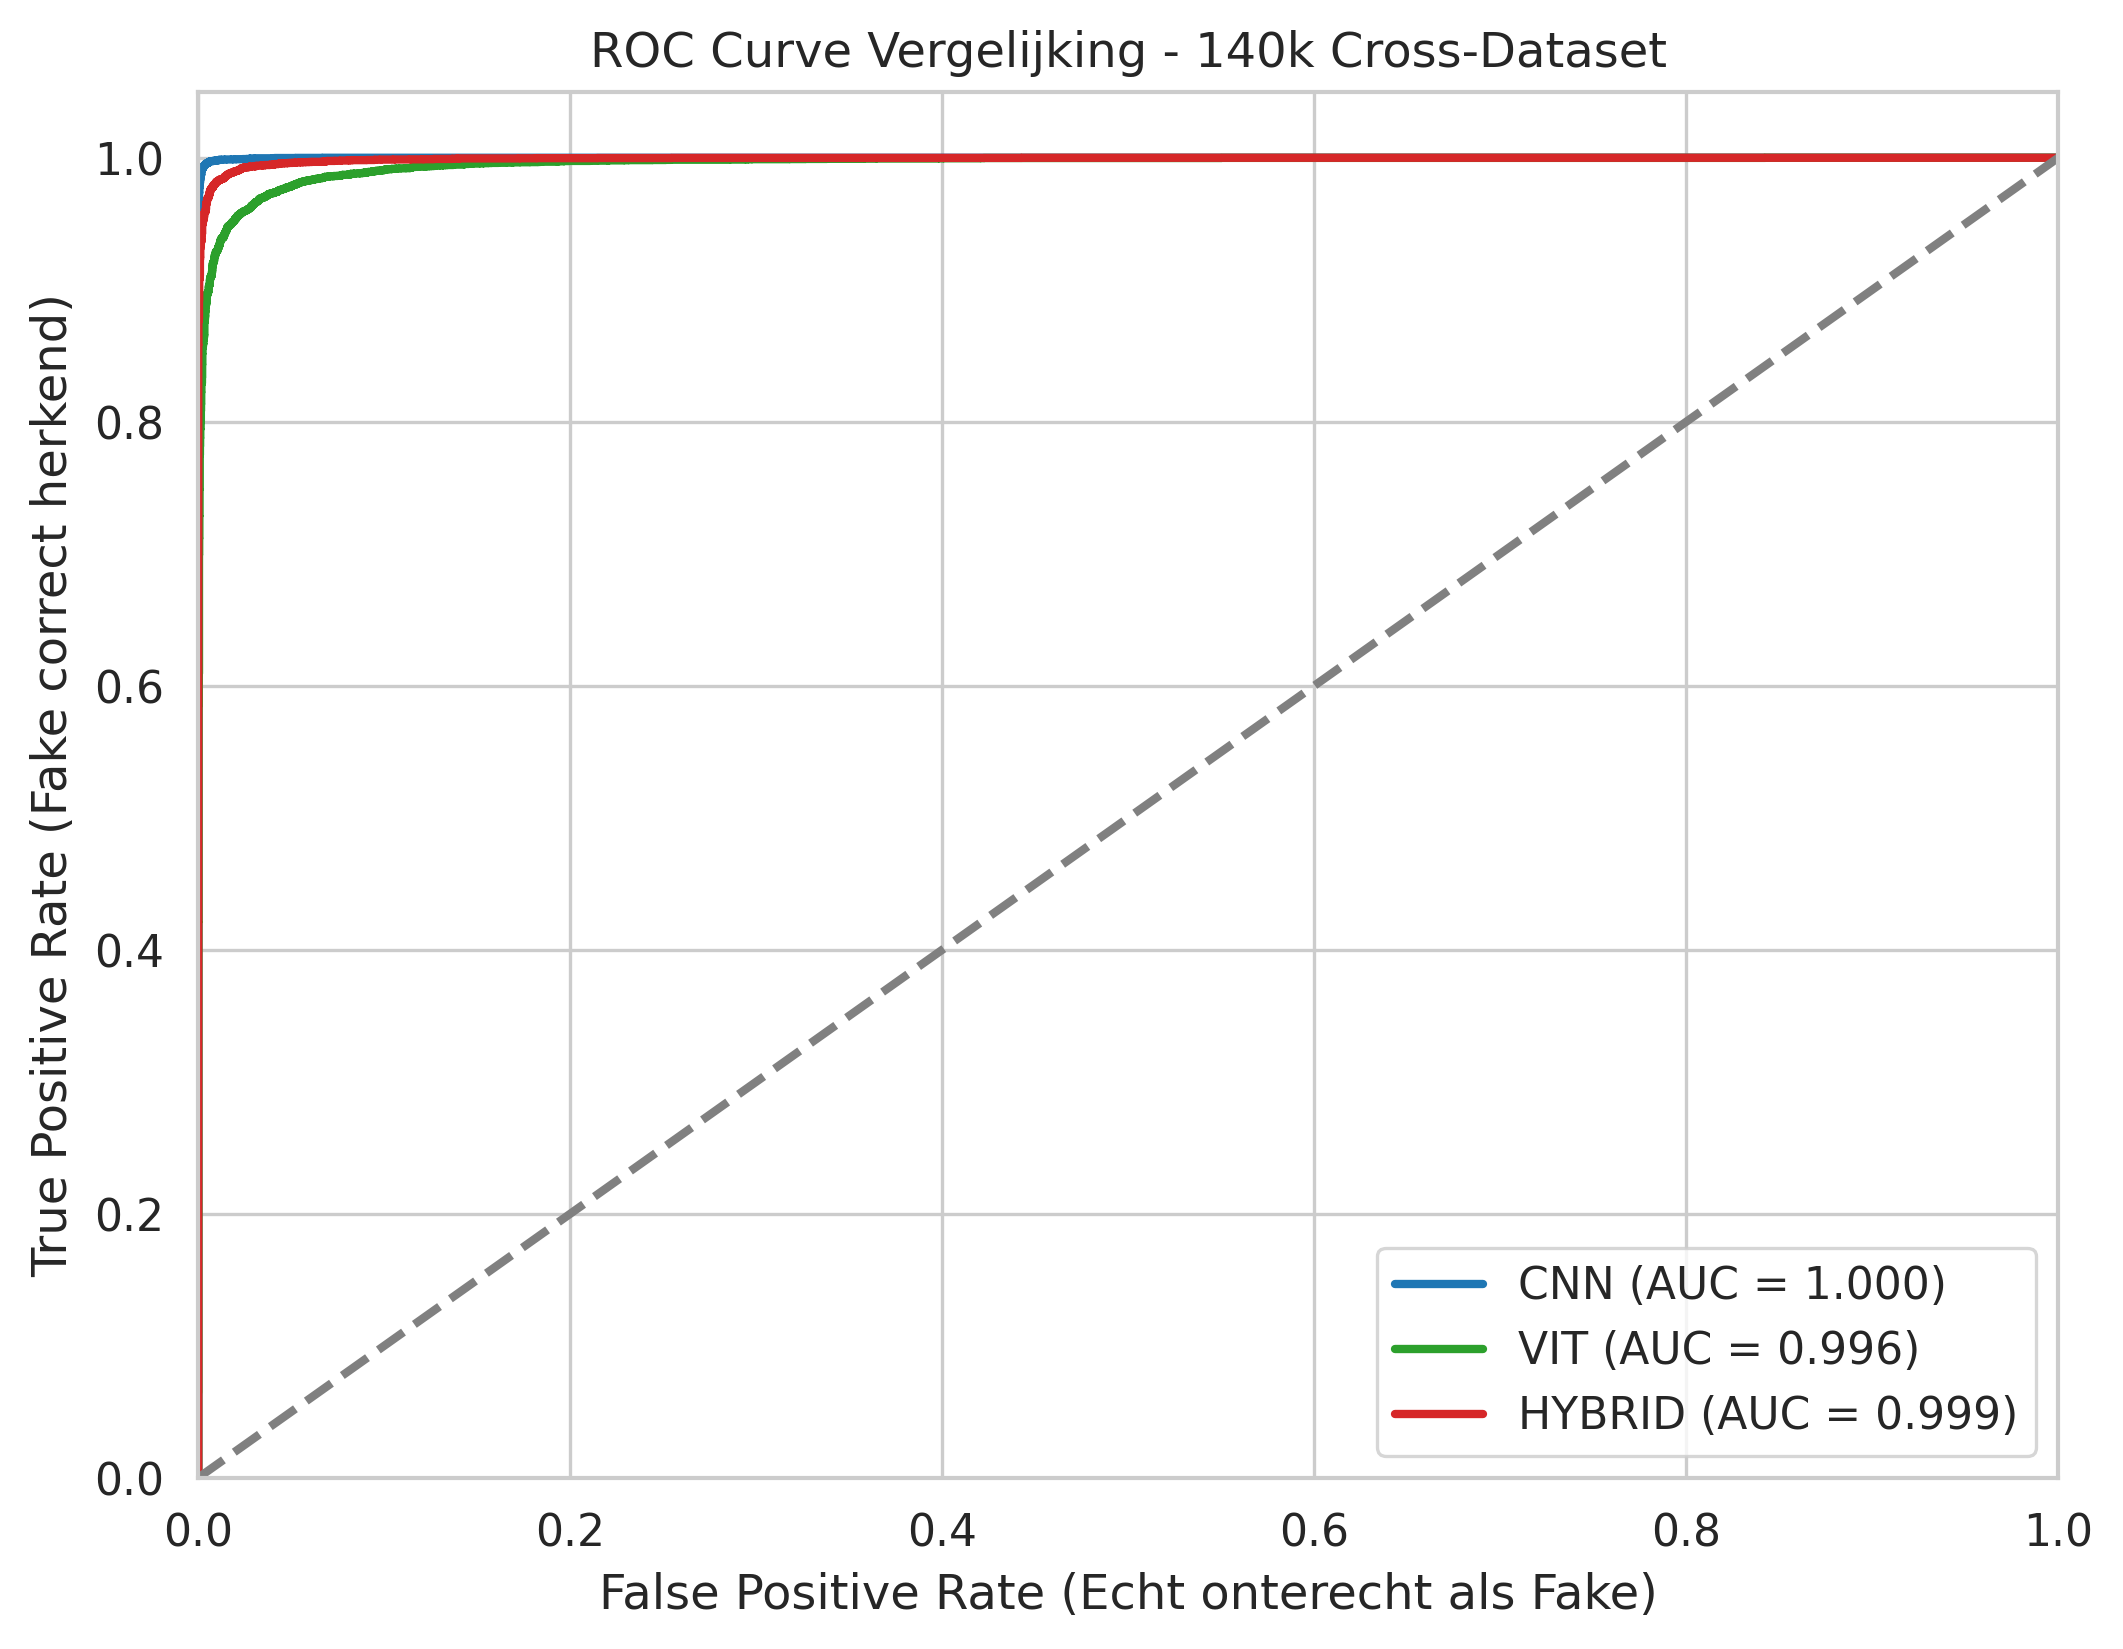
\includegraphics[width=\textwidth]{../ipynb_output/roc_pr/ROC_140k.png}
        \centerline{\scriptsize (a) ROC-curve op 140k}
    \end{minipage}
    \hfill
    \begin{minipage}{0.48\textwidth}
        \centering
        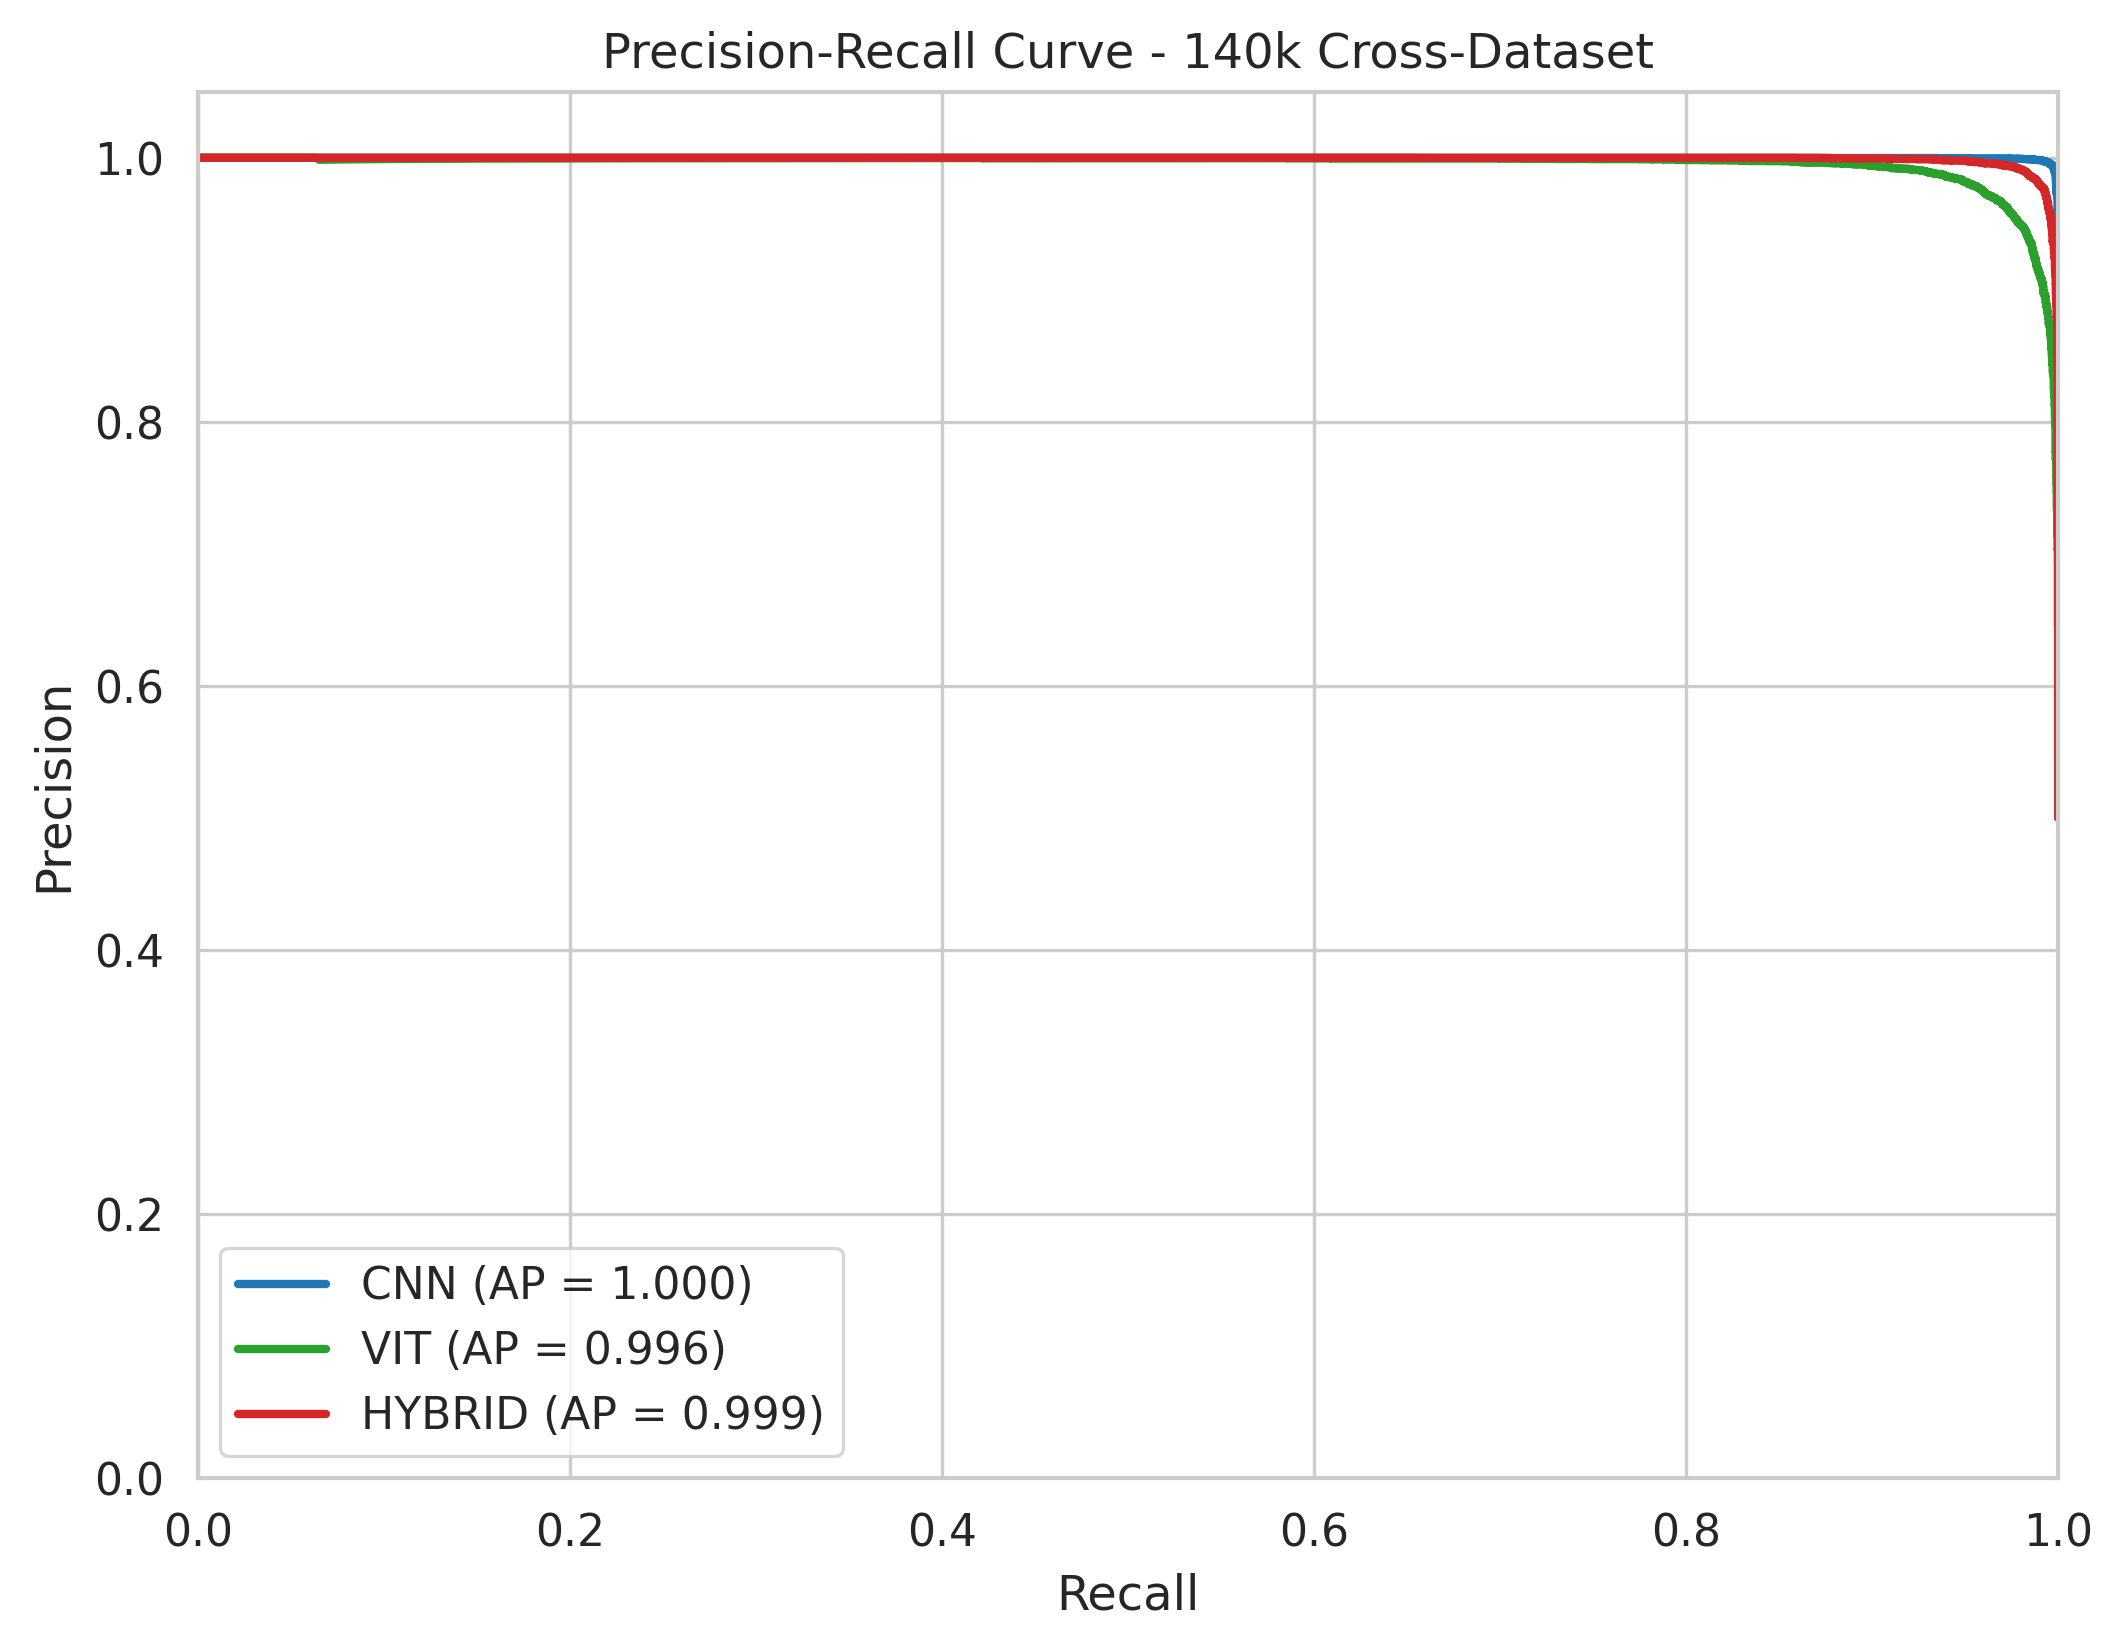
\includegraphics[width=\textwidth]{../ipynb_output/roc_pr/PR_140k.png}
        \centerline{\scriptsize (b) PR-curve op 140k}
    \end{minipage}
    \caption[ROC- en PR-curves op 140k]{ROC- en PR-curves voor de 140k Real and Fake Faces dataset.}
    \label{fig:roc_pr_140k}
\end{figure}

De confusion matrices (Figuur \ref{fig:confusion_matrices}) en de numerieke foutenstructuur tonen verschillen tussen datasets. Op DeepDetect werden substantiele aantallen false positives geregistreerd (zie Tabel/figuren), terwijl op de externe 140k-dataset de foutenstructuur aanzienlijk anders was. Dit wijst op dataset-specifieke artefacten en benadrukt het belang van cross-dataset evaluatie voor robuustheidsinschatting.

\begin{figure}[H]
    \centering
    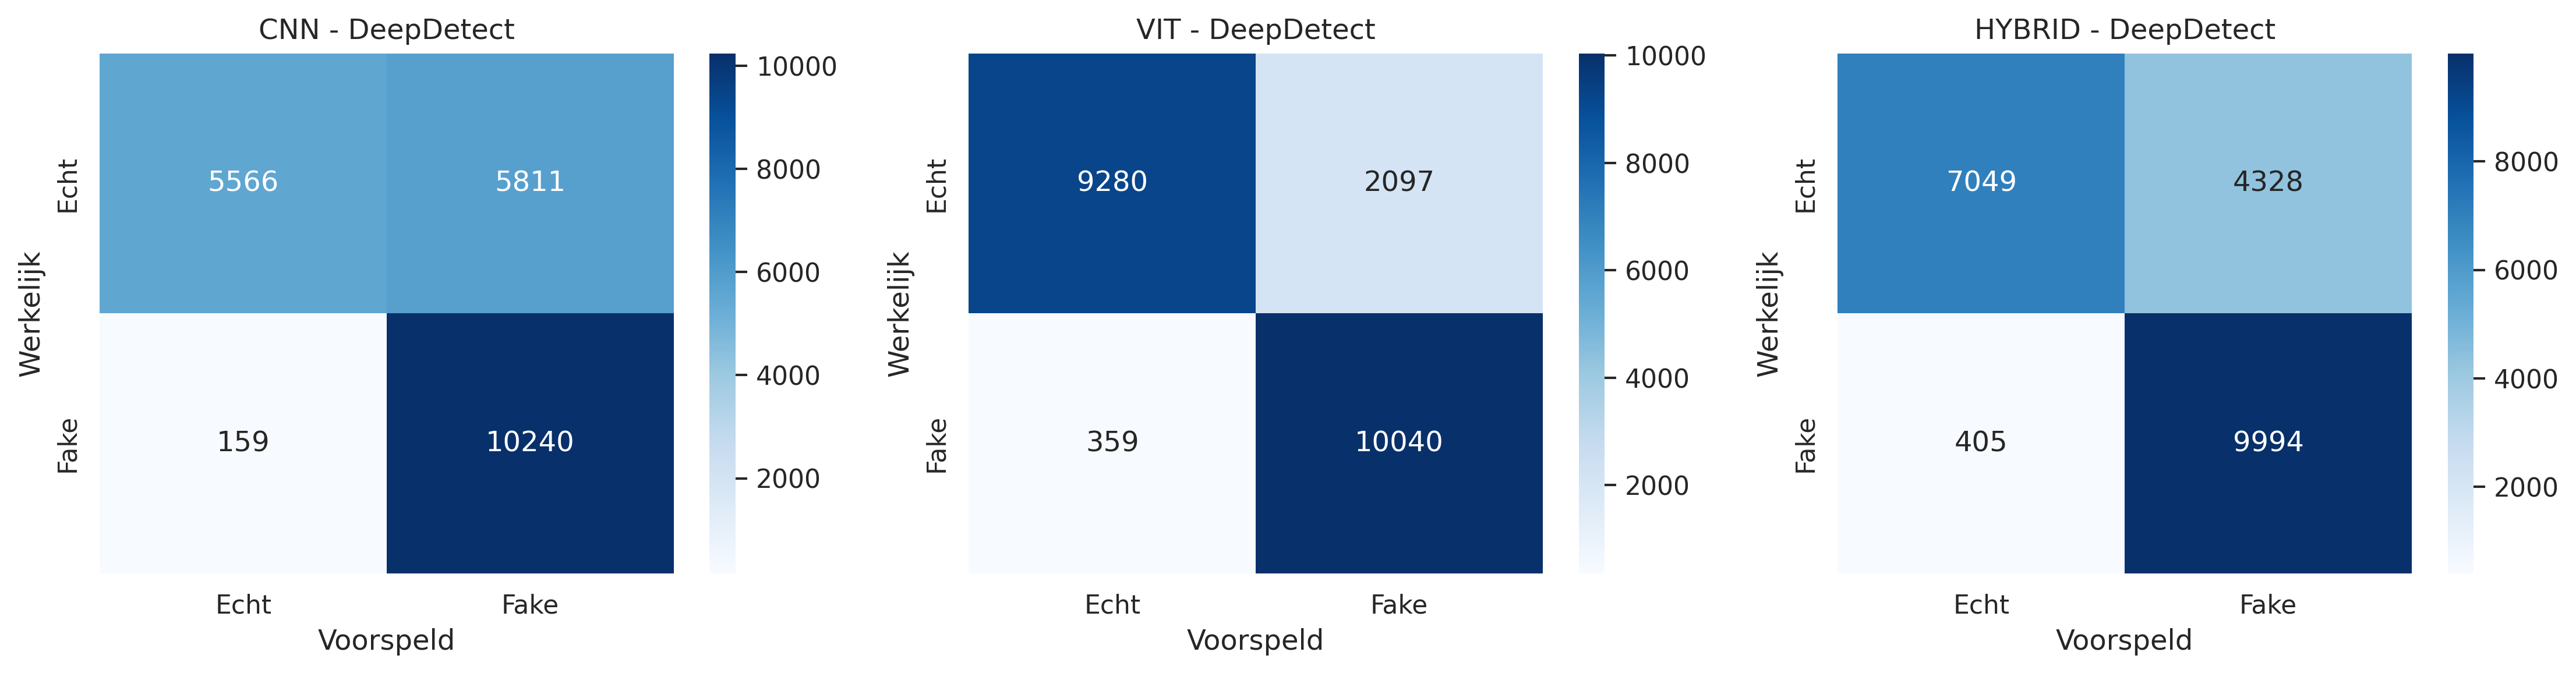
\includegraphics[width=0.9\textwidth]{../ipynb_output/confusion_matrices/CM_DeepDetect.png}
    \centerline{\small (a) DeepDetect-2025}
    
    \vspace{1cm}
    
    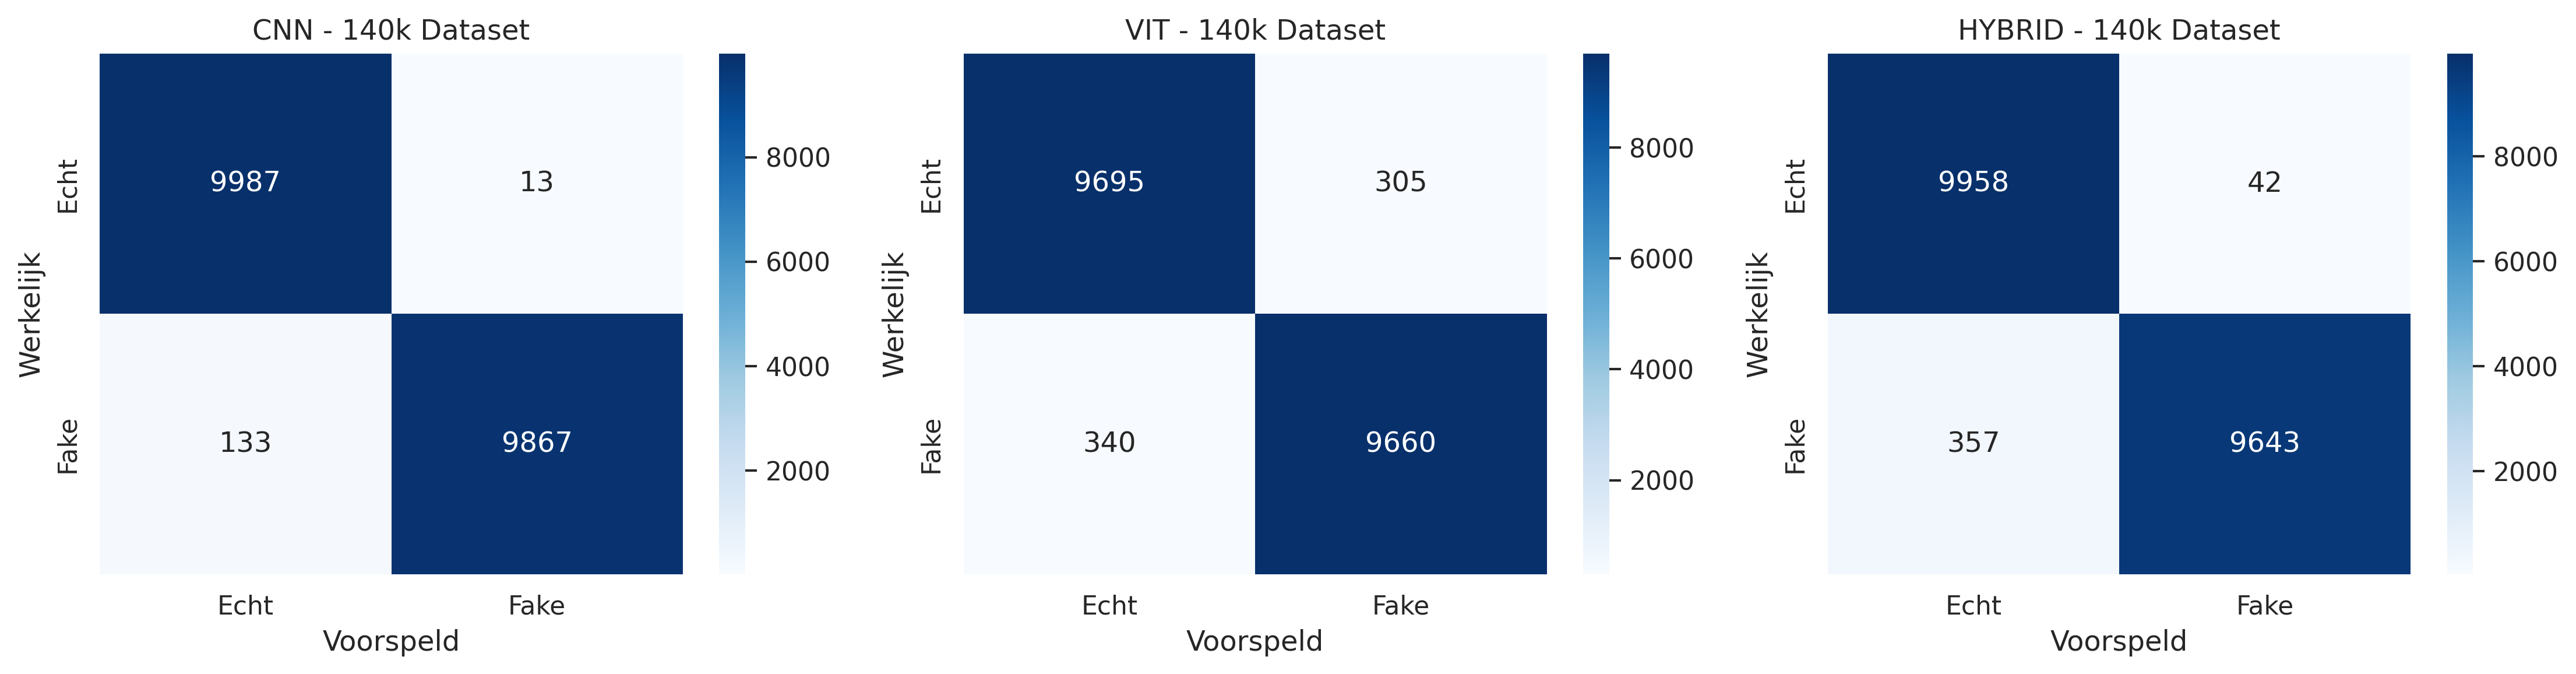
\includegraphics[width=0.9\textwidth]{../ipynb_output/confusion_matrices/CM_140k.png}
    \centerline{\small (b) 140k Real and Fake Faces}
    
    \caption[Confusion matrices voor DeepDetect-2025 en 140k.]{Confusion matrices voor beide datasets.}
    \label{fig:confusion_matrices}
\end{figure}

\begin{figure}[H]
    \centering
    \begin{minipage}{0.48\textwidth}
        \centering
        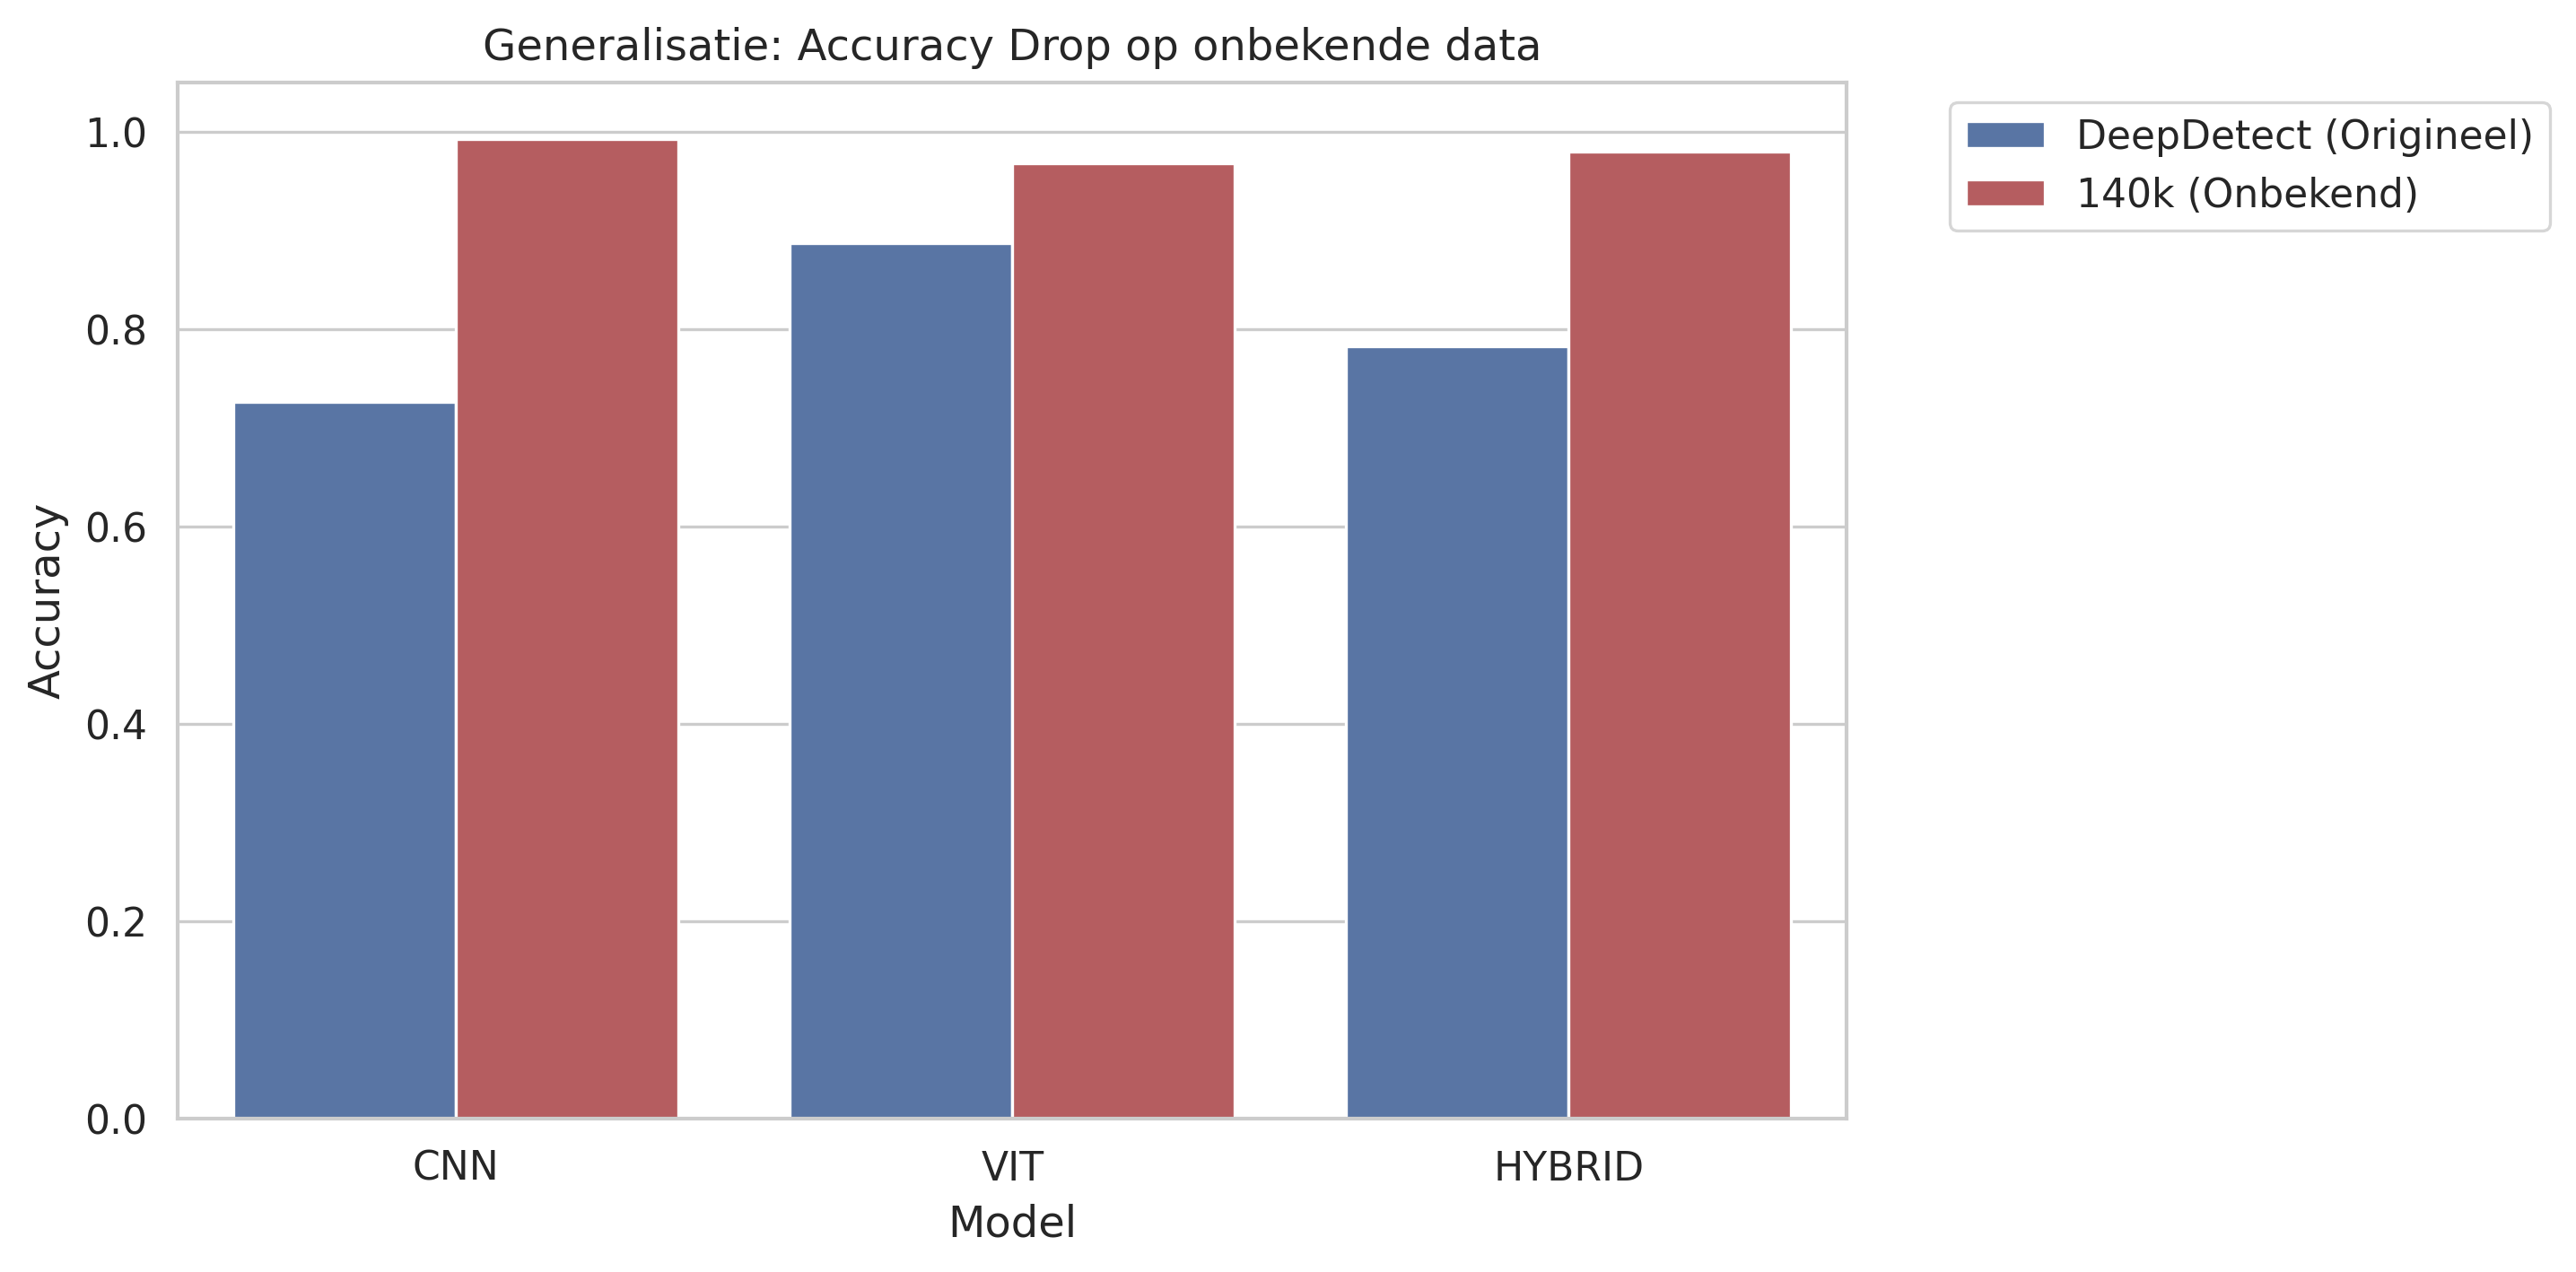
\includegraphics[width=\textwidth]{../ipynb_output/metrics/Accuracy_Drop.png}
        \centerline{\scriptsize (a) Accuracy vergelijking}
    \end{minipage}
    \hfill
    \begin{minipage}{0.48\textwidth}
        \centering
        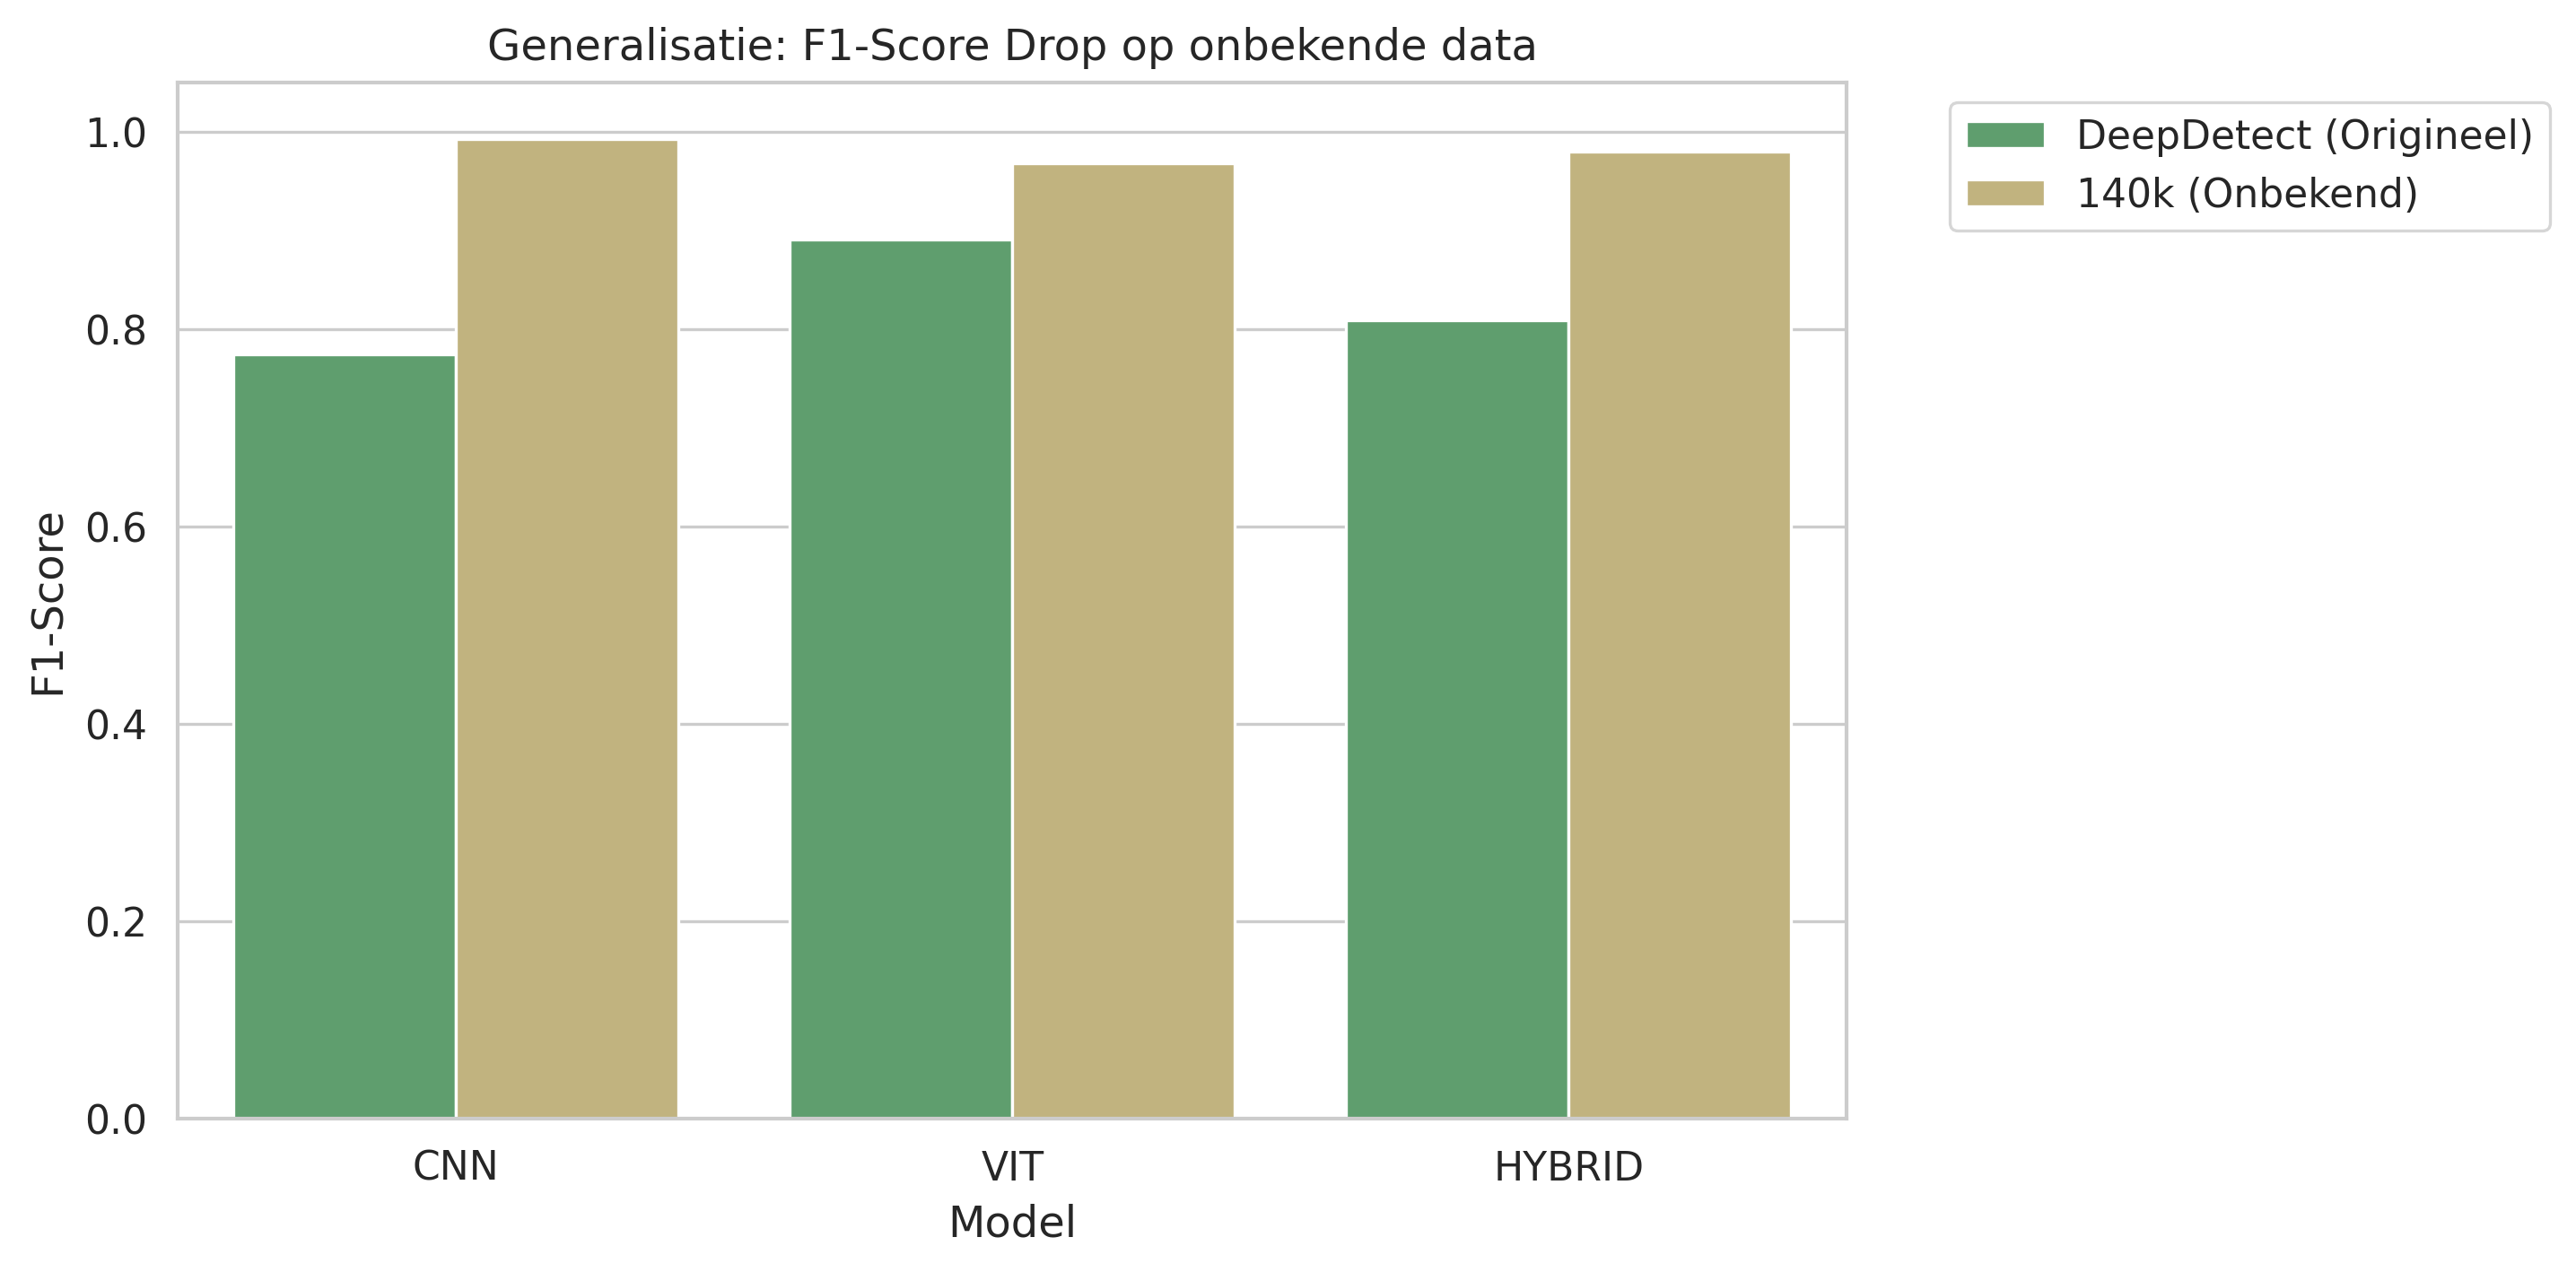
\includegraphics[width=\textwidth]{../ipynb_output/metrics/F1_Drop.png}
        \centerline{\scriptsize (b) F1-score vergelijking}
    \end{minipage}
    \caption[Accuracy- en F1-vergelijking tussen datasets]{Vergelijking van accuracy en F1-score op DeepDetect en 140k.}
    \label{fig:accuracy_f1_comparison}
\end{figure}

\section{Robuustheid onder JPEG-Compressie}
\label{sec:jpeg_robustness}

Om real-world compressie-effecten te simuleren is een JPEG-degradatie-experiment uitgevoerd. Het script dat de degradatie toepast staat in de codebase en de resultaten zijn samengebracht in de F1-vs-JPEG-kwaliteit grafiek.

\begin{listing}[H]
    \inputminted[fontsize=\footnotesize, linenos, frame=lines]{python}{code/jpeg_compression.py}
    \caption{Python script voor het JPEG-robuustheidsexperiment.}
    \label{lst:results_jpeg_compression}
\end{listing}

\begin{figure}[H]
    \centering
    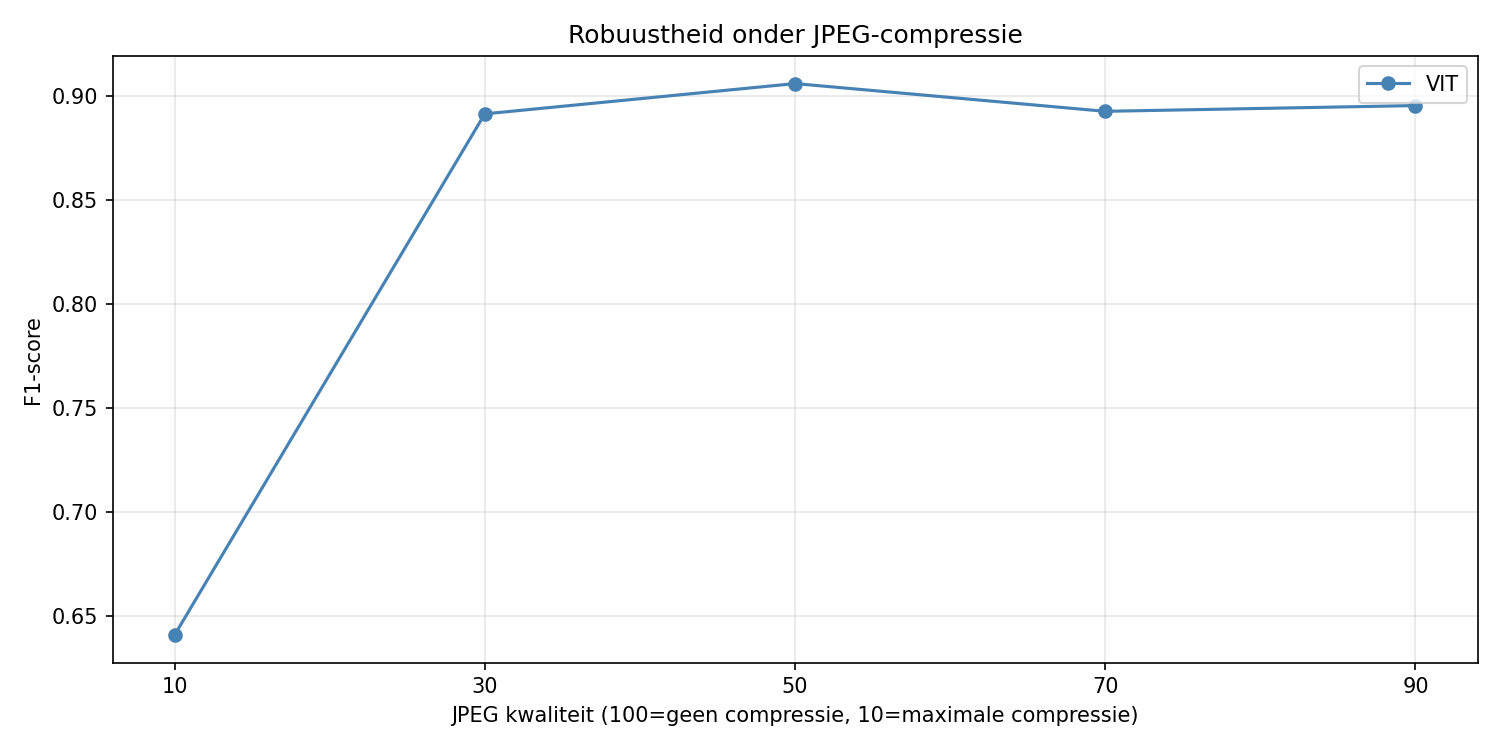
\includegraphics[width=0.9\textwidth]{../ipynb_output/ViT_results/robustness_jpeg.png}
    \caption[Robuustheid onder JPEG-compressie]{F1-score als functie van JPEG-kwaliteit voor de drie modellen.}
    \label{fig:robustness_jpeg}
\end{figure}

\section{Visuele Foutanalyse via Grad-CAM++}
\label{sec:gradcam_results}

Grad-CAM++ heatmaps zijn gegenereerd voor representatieve voorbeelden uit de vier categorieën van de confusion matrix (TP, TN, FP, FN) voor elk model. Deze heatmaps helpen te interpreteren welke regio's de beslissingen sturen.

\begin{listing}[H]
    \inputminted[fontsize=\footnotesize, linenos, frame=lines]{python}{code/gradcam_impl.py}
    \caption{Python script voor de Grad-CAM++ implementatie.}
    \label{lst:results_gradcam_impl}
\end{listing}

\begin{figure}[H]
    \centering
    % === CNN RIJ ===
    \begin{minipage}{0.24\textwidth}
        \centering
        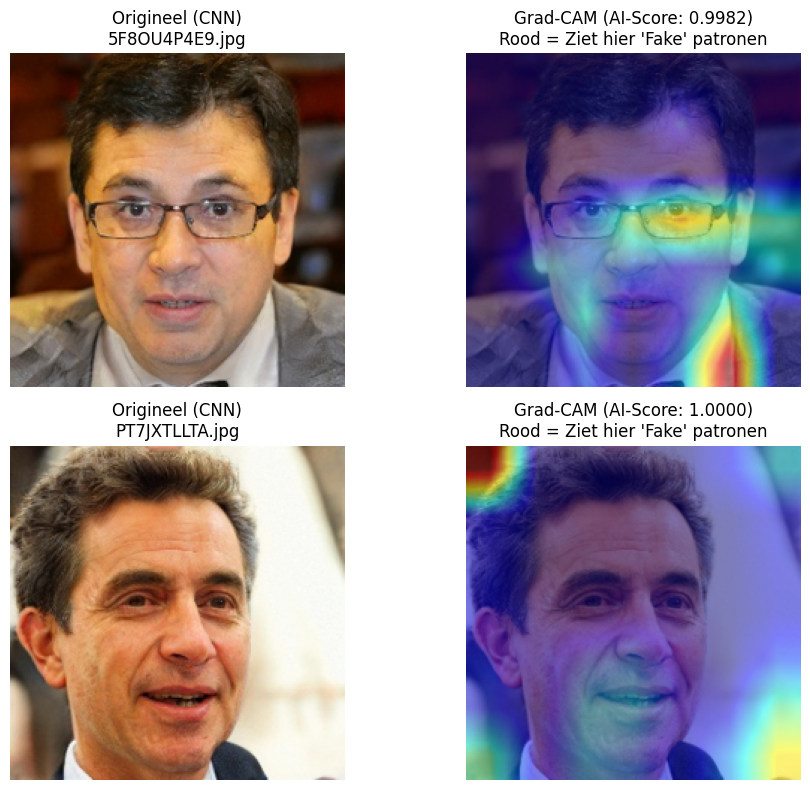
\includegraphics[width=\textwidth]{../ipynb_output/Heatmaps/CNN/true_positive.png}
        {\scriptsize (a) CNN TP}
    \end{minipage}
    \hfill
    \begin{minipage}{0.24\textwidth}
        \centering
        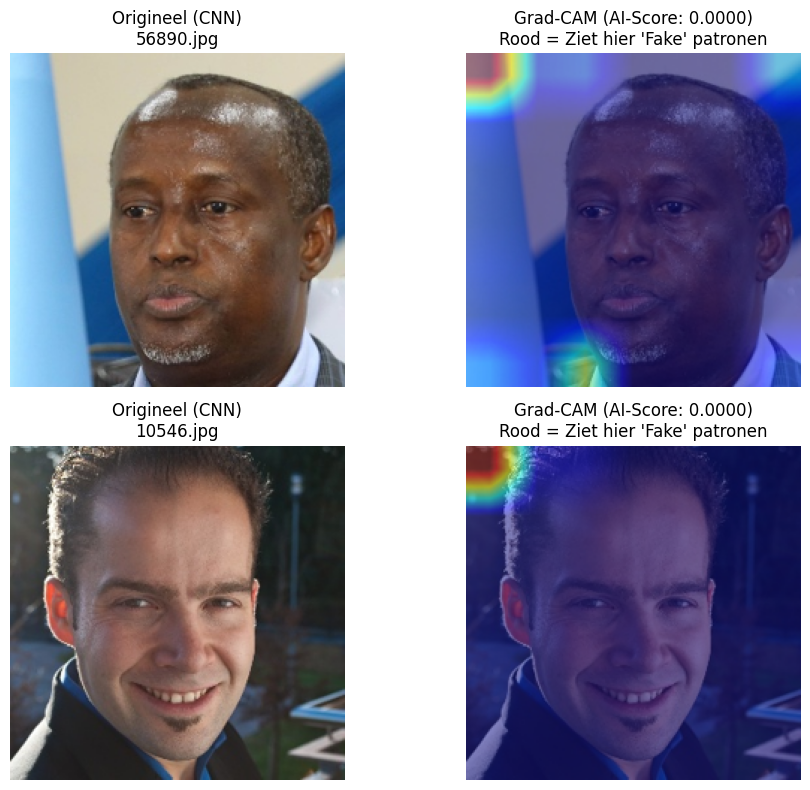
\includegraphics[width=\textwidth]{../ipynb_output/Heatmaps/CNN/true_negative.png}
        {\scriptsize (b) CNN TN}
    \end{minipage}
    \hfill
    \begin{minipage}{0.24\textwidth}
        \centering
        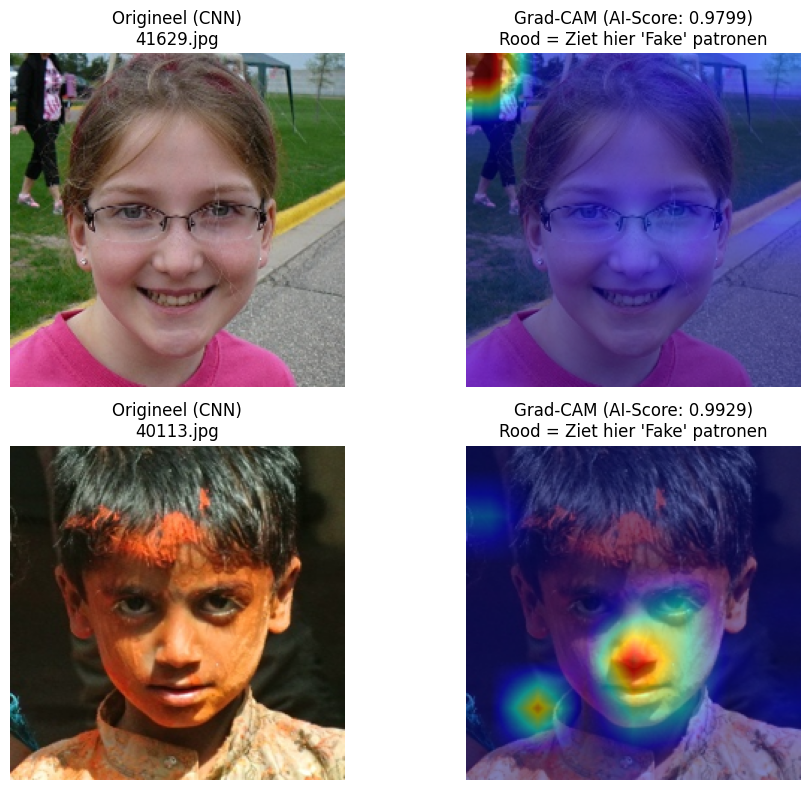
\includegraphics[width=\textwidth]{../ipynb_output/Heatmaps/CNN/false_positive.png}
        {\scriptsize (c) CNN FP}
    \end{minipage}
    \hfill
    \begin{minipage}{0.24\textwidth}
        \centering
        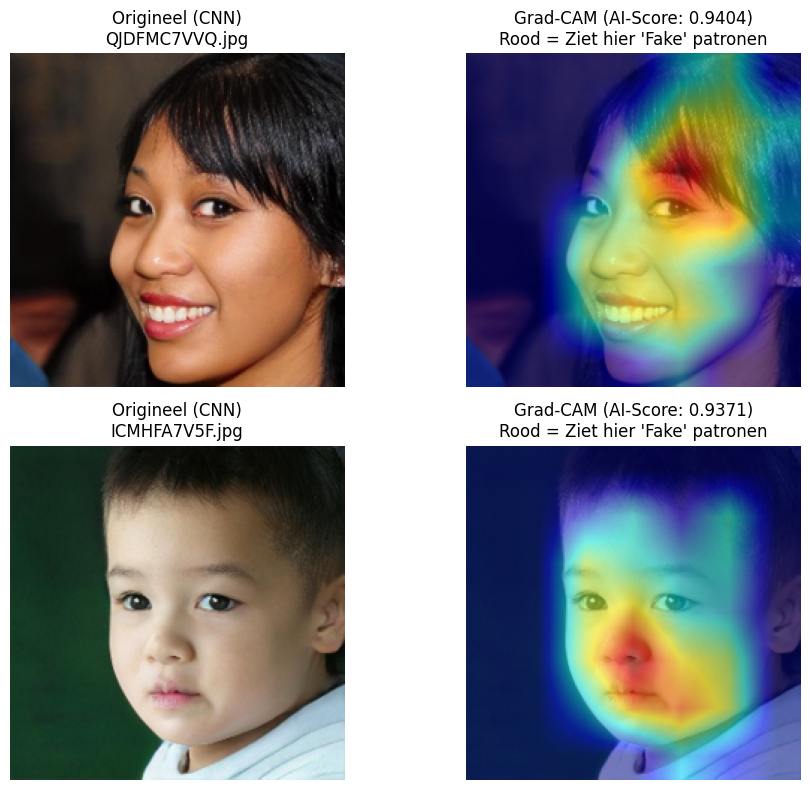
\includegraphics[width=\textwidth]{../ipynb_output/Heatmaps/CNN/false_negative.png}
        {\scriptsize (d) CNN FN}
    \end{minipage}

    \vspace{0.8cm}

    % === ViT RIJ ===
    \begin{minipage}{0.24\textwidth}
        \centering
        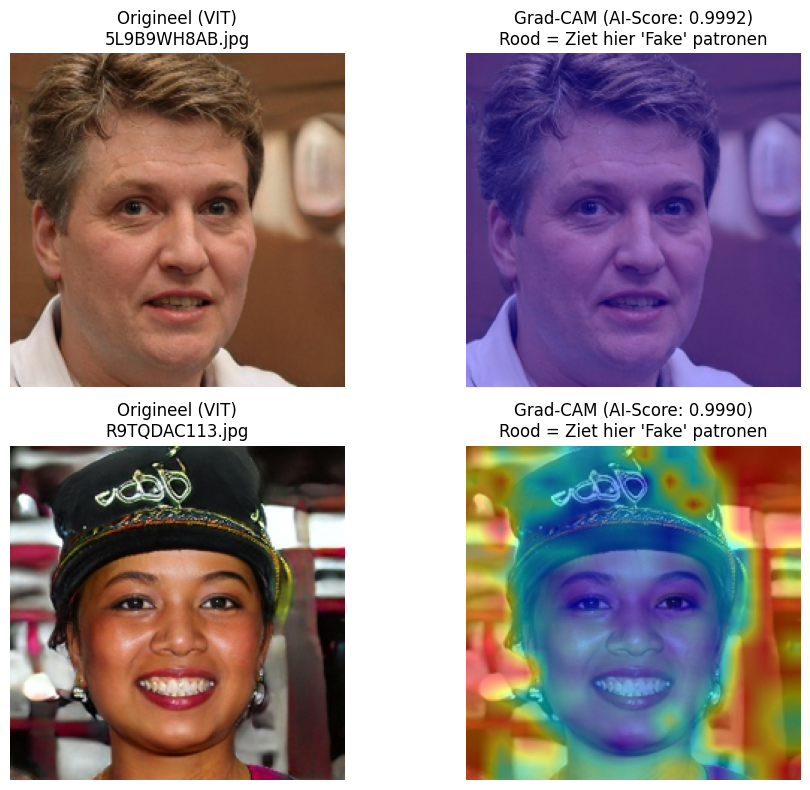
\includegraphics[width=\textwidth]{../ipynb_output/Heatmaps/VIT/true_positive.png}
        {\scriptsize (e) ViT TP}
    \end{minipage}
    \hfill
    \begin{minipage}{0.24\textwidth}
        \centering
        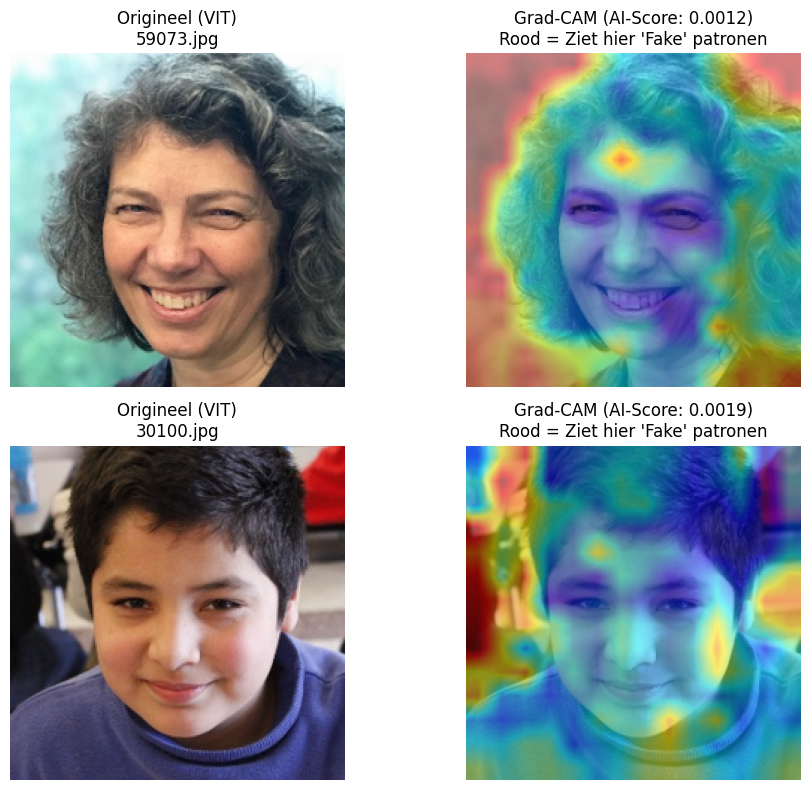
\includegraphics[width=\textwidth]{../ipynb_output/Heatmaps/VIT/true_negative.png}
        {\scriptsize (f) ViT TN}
    \end{minipage}
    \hfill
    \begin{minipage}{0.24\textwidth}
        \centering
        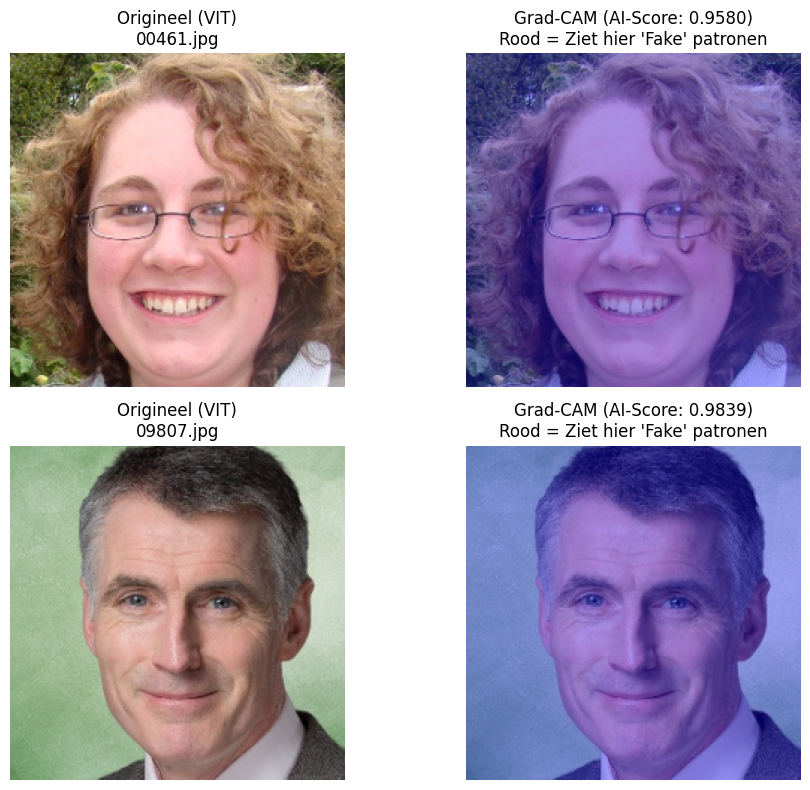
\includegraphics[width=\textwidth]{../ipynb_output/Heatmaps/VIT/false_positive.png}
        {\scriptsize (g) ViT FP}
    \end{minipage}
    \hfill
    \begin{minipage}{0.24\textwidth}
        \centering
        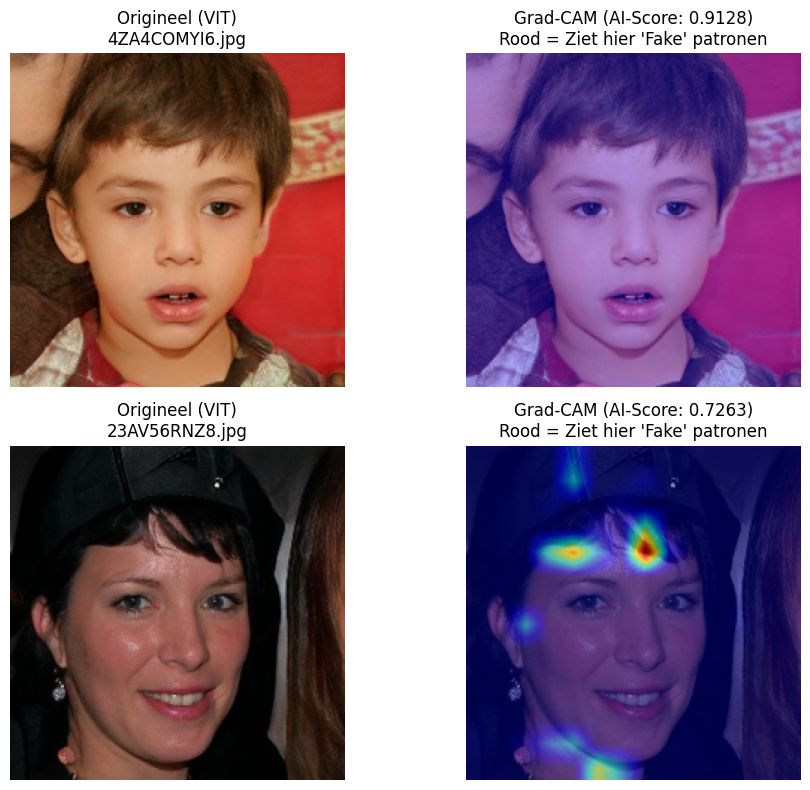
\includegraphics[width=\textwidth]{../ipynb_output/Heatmaps/VIT/false_negative.png}
        {\scriptsize (h) ViT FN}
    \end{minipage}

    \vspace{0.8cm}

    % === HYBRIDE RIJ ===
    \begin{minipage}{0.24\textwidth}
        \centering
        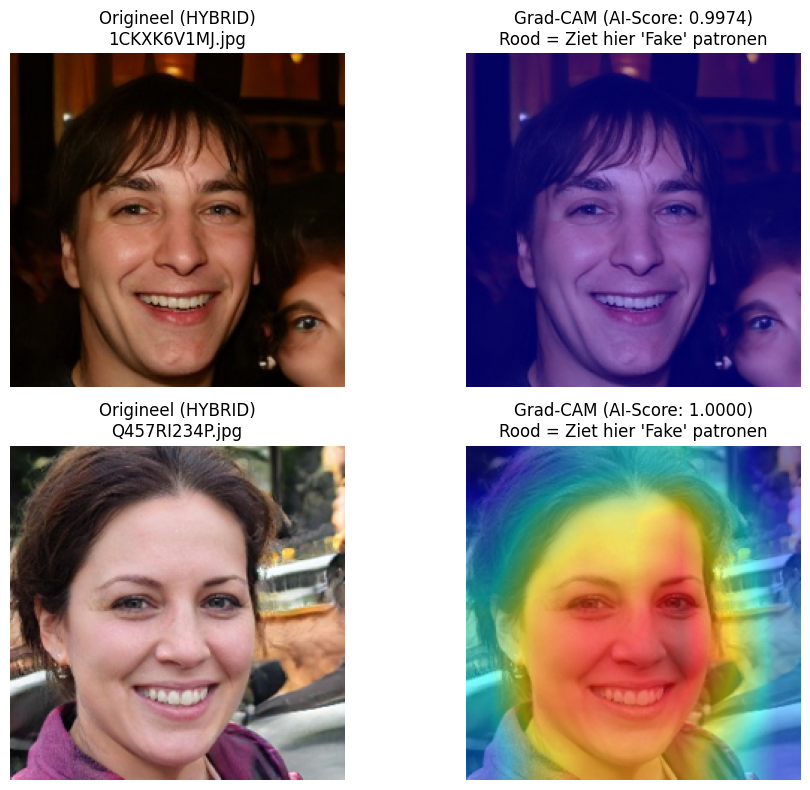
\includegraphics[width=\textwidth]{../ipynb_output/Heatmaps/HYBRID/true_positive.png}
        {\scriptsize (i) Hybride TP}
    \end{minipage}
    \hfill
    \begin{minipage}{0.24\textwidth}
        \centering
        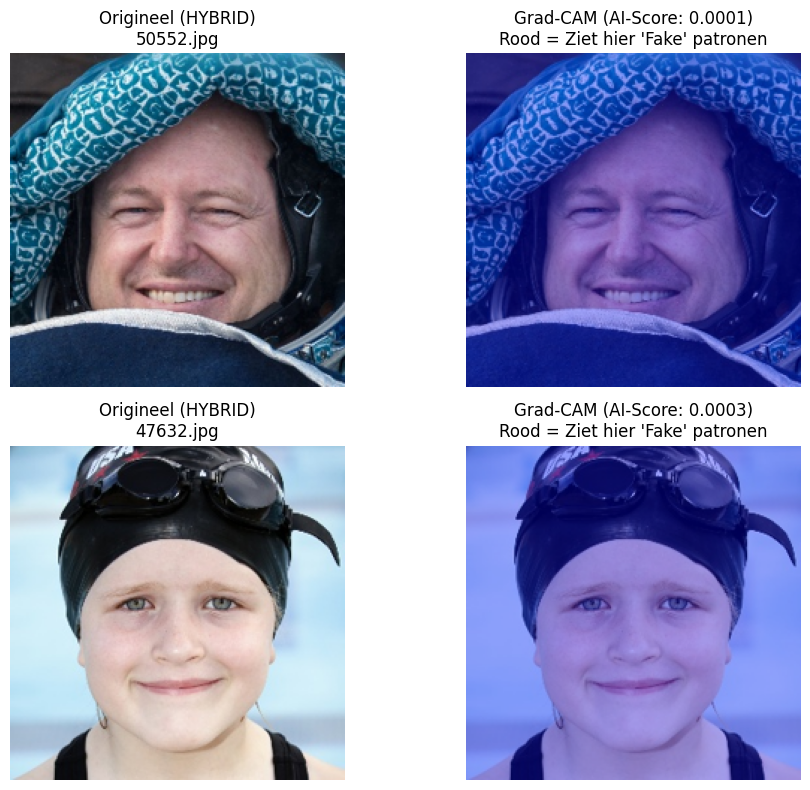
\includegraphics[width=\textwidth]{../ipynb_output/Heatmaps/HYBRID/true_negative.png}
        {\scriptsize (j) Hybride TN}
    \end{minipage}
    \hfill
    \begin{minipage}{0.24\textwidth}
        \centering
        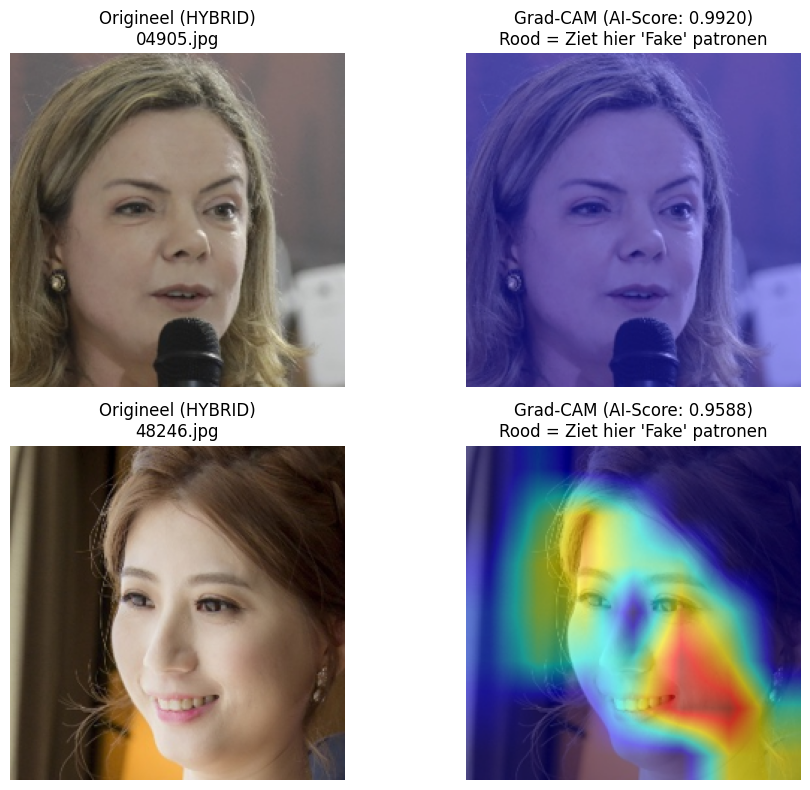
\includegraphics[width=\textwidth]{../ipynb_output/Heatmaps/HYBRID/false_positive.png}
        {\scriptsize (k) Hybride FP}
    \end{minipage}
    \hfill
    \begin{minipage}{0.24\textwidth}
        \centering
        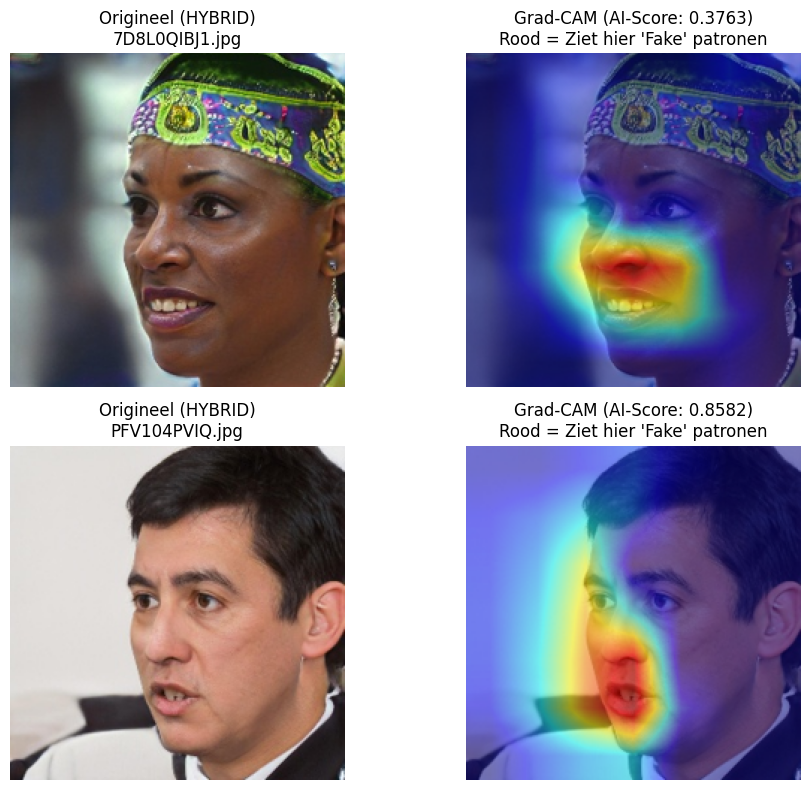
\includegraphics[width=\textwidth]{../ipynb_output/Heatmaps/HYBRID/false_negative.png}
        {\scriptsize (l) Hybride FN}
    \end{minipage}

    \caption[Grad-CAM++ heatmaps voor alle modellen]{Grad-CAM++ heatmaps voor CNN, ViT en Hybride modellen (TP/TN/FP/FN voorbeelden).}
    \label{fig:all_gradcam_heatmaps}
\end{figure}

\subsection{Most Confident Errors}

Het subsetje van "most confident errors" (fouten met hoge voorspelde kans) is geëxtraheerd en visueel geanalyseerd; het gebruikte script staat in de codebase.

\begin{listing}[H]
    \inputminted[fontsize=\footnotesize, linenos, frame=lines]{python}{code/confident_errors.py}
    \caption{Python script voor de analyse van most confident errors.}
    \label{lst:results_confident_errors}
\end{listing}

\section{Beslissingsdrempel Optimalisatie}

De threshold-analyse is uitgevoerd door de F1-score te evalueren op een raster van mogelijke drempels. De resulterende curve en de per-model optimale drempels worden in Figuur \ref{fig:threshold_analysis} samengebracht.

\begin{listing}[H]
    \inputminted[fontsize=\footnotesize, linenos, frame=lines]{python}{code/threshold_optim.py}
    \caption{Python script voor de optimalisatie van de beslissingsdrempel.}
    \label{lst:results_threshold_optim}
\end{listing}

\begin{figure}[H]
    \centering
    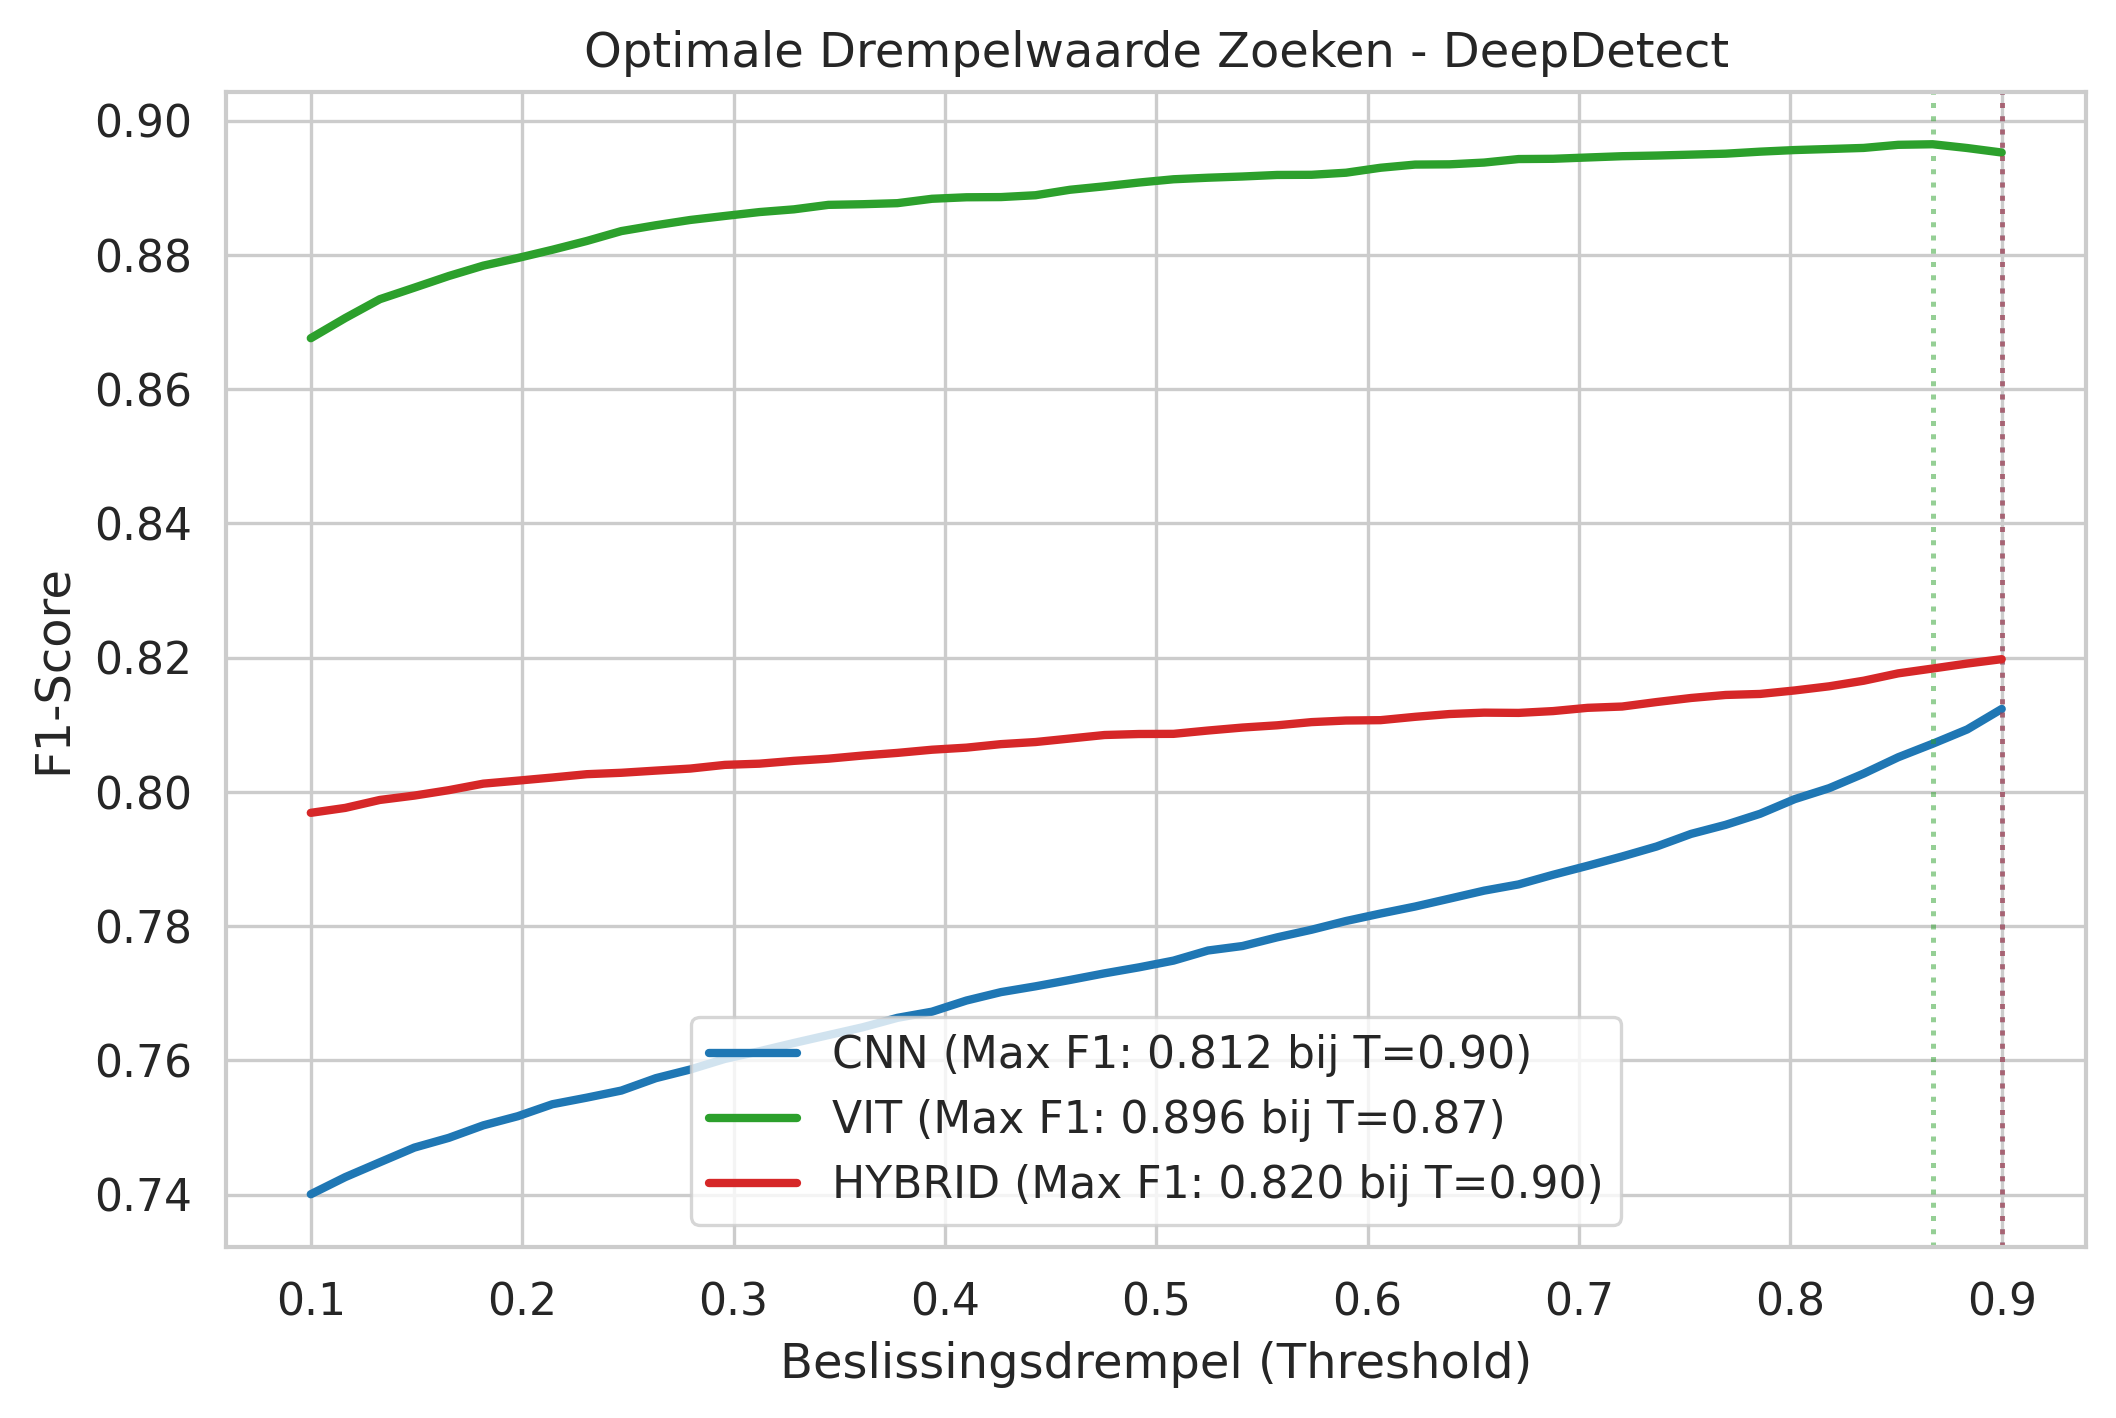
\includegraphics[width=0.9\textwidth]{../ipynb_output/metrics/F1_Threshold_DeepDetect.png}
    \caption[Threshold-optimalisatie op DeepDetect]{F1-score als functie van de beslissingsdrempel voor de drie modellen; de optimale drempels zijn aangegeven per model.}
    \label{fig:threshold_analysis}
\end{figure}

% einde resultaten
